\documentclass[aspectratio=169,10pt]{beamer}

\usetheme{metropolis}
\metroset{
  progressbar=frametitle,
  sectionpage=progressbar,
  numbering=fraction,
  block=fill
}

\usepackage{fontspec}
\usepackage{xeCJK}
\setsansfont{TeX Gyre Heros}
\setmonofont{Latin Modern Mono}
\setCJKsansfont[BoldFont=FandolHei-Bold.otf]{FandolHei-Regular.otf}
\setCJKmonofont{FandolFang-Regular.otf}

\usepackage{amsmath,amssymb,mathtools}
\usepackage{booktabs,tabularx,array,multirow}
\usepackage{tikz}
\usetikzlibrary{arrows.meta,positioning,fit,calc,shapes.geometric,backgrounds}
\usepackage{pgfplots}
\pgfplotsset{compat=1.18}
\usepackage{listings}
\usepackage{ragged2e}
\usepackage{graphicx}
\usepackage{hyperref}
\usepackage{xurl}
\usepackage[backend=biber,style=numeric-comp,sorting=none,maxbibnames=3,giveninits=true]{biblatex}
\addbibresource{intelligence_agent_references.bib}

\definecolor{Ink}{HTML}{172033}
\definecolor{Navy}{HTML}{163A5F}
\definecolor{Cyan}{HTML}{00A6A6}
\definecolor{Blue}{HTML}{2F6BFF}
\definecolor{Green}{HTML}{1B9E77}
\definecolor{Amber}{HTML}{E69F00}
\definecolor{Red}{HTML}{D1495B}
\definecolor{Purple}{HTML}{7251B5}
\definecolor{Paper}{HTML}{F7F9FC}
\definecolor{Slate}{HTML}{5B6577}
\definecolor{SoftBlue}{HTML}{E9F1FF}
\definecolor{SoftGreen}{HTML}{E9F7F2}
\definecolor{SoftAmber}{HTML}{FFF4D9}
\definecolor{SoftRed}{HTML}{FCECEF}

\setbeamercolor{normal text}{fg=Ink,bg=white}
\setbeamercolor{alerted text}{fg=Red}
\setbeamercolor{frametitle}{fg=white,bg=Navy}
\setbeamercolor{progress bar}{fg=Cyan,bg=SoftBlue}
\setbeamercolor{title separator}{fg=Cyan}
\setbeamercolor{block title}{fg=white,bg=Navy}
\setbeamercolor{block body}{fg=Ink,bg=Paper}
\setbeamercolor{block title alerted}{fg=white,bg=Red}
\setbeamercolor{block body alerted}{fg=Ink,bg=SoftRed}
\setbeamercolor{block title example}{fg=white,bg=Green}
\setbeamercolor{block body example}{fg=Ink,bg=SoftGreen}
\setbeamerfont{title}{size=\Large,series=\bfseries}
\setbeamerfont{subtitle}{size=\scriptsize}
\setbeamerfont{author}{size=\scriptsize}
\setbeamerfont{institute}{size=\tiny}
\setbeamertemplate{navigation symbols}{}
\setbeamertemplate{caption}[numbered]

\newcommand{\impl}{\textcolor{Green}{\scriptsize\bfseries [当前实现]}}
\newcommand{\obs}{\textcolor{Blue}{\scriptsize\bfseries [运行观测]}}
\newcommand{\risk}{\textcolor{Red}{\scriptsize\bfseries [风险/限制]}}
\newcommand{\proposal}{\textcolor{Purple}{\scriptsize\bfseries [改进建议]}}
\newcommand{\research}{\textcolor{Amber}{\scriptsize\bfseries [研究假设]}}
\newcommand{\pathcode}[1]{\texttt{\detokenize{#1}}}
\newcommand{\smallsource}[1]{\vspace{0.15em}\par{\tiny\color{Slate}证据：#1}}
\newcommand{\metric}[2]{\begin{minipage}[t]{0.215\textwidth}\centering{\Large\bfseries\color{Navy}#1}\\[-0.15em]{\scriptsize #2}\end{minipage}}
\newcommand{\yes}{\textcolor{Green}{\bfseries\checkmark}}
\newcommand{\no}{\textcolor{Red}{\bfseries--}}

\lstset{
  language=Python,
  basicstyle=\ttfamily\scriptsize,
  keywordstyle=\color{Blue}\bfseries,
  stringstyle=\color{Green},
  commentstyle=\color{Slate}\itshape,
  showstringspaces=false,
  columns=fullflexible,
  keepspaces=true,
  frame=single,
  rulecolor=\color{SoftBlue},
  backgroundcolor=\color{Paper},
  breaklines=true,
  tabsize=4
}

\AtBeginSection[]{
  \begin{frame}[plain,noframenumbering]
    \sectionpage
  \end{frame}
}

\title{LLM 安全情报采集智能体：\newline 源码审计、运行证据与研究路线}
\subtitle{架构 - 原理 - 算法 - 数理解释 - 代码映射 - 运行结果 - DMAIC - 学术化}
\author{项目技术报告}
\institute{基于当前工作树与 2026-07-15 本机运行快照}
\date{2026 年 7 月 15 日}

\begin{document}

\begin{frame}[plain]
  \vfill
  {\Large\bfseries\color{Navy}\inserttitle\par}
  \vspace{0.35em}
  {\color{Cyan}\rule{0.26\linewidth}{2pt}\par}
  \vspace{0.65em}
  {\scriptsize\insertsubtitle\par}
  \vfill
  {\scriptsize\insertauthor\par}
  \vspace{0.25em}
  {\tiny\insertinstitute\par}
  \vspace{0.25em}
  {\tiny\insertdate\par}
  \vfill
\end{frame}

\section{报告范围与结论}

\begin{frame}{如何阅读这份报告}
\begin{columns}[T,onlytextwidth]
\column{0.31\textwidth}
\begin{block}{第一层：事实}
当前 \pathcode{backend/} 源码、配置、测试、Mongo 和 trace；所有“已实现”结论可回到文件定位。
\end{block}
\column{0.31\textwidth}
\begin{block}{第二层：解释}
把控制流、状态、公式和数据口径连起来，解释为何系统会产生当前运行结果。
\end{block}
\column{0.31\textwidth}
\begin{block}{第三层：设计}
DMAIC 与论文实验是未来方案，使用 \proposal/\research 标识，不冒充已有能力。
\end{block}
\end{columns}

\vspace{0.5em}
\begin{center}
\impl\ 当前代码 \quad
\obs\ 真实运行 \quad
\risk\ 已识别限制 \quad
\proposal\ 工程改进 \quad
\research\ 待验证命题
\end{center}

\smallsource{完整证据索引：\pathcode{report/code_evidence_matrix.md}；运行快照：\pathcode{report/runtime_snapshot.json}}
\end{frame}

\begin{frame}{执行摘要：系统已可运行，但“有效覆盖”尚未闭环}
\begin{columns}[T,onlytextwidth]
\column{0.32\textwidth}
\begin{exampleblock}{已经成立}
\begin{itemize}
  \item 四个真实源与统一 DTO
  \item SDK tool loop + 本地 MCP 白名单
  \item 相关性三层管线
  \item Mongo 全局去重、trace 与 item-KG 交接
  \item adaptive 的 CorpusGap、UCB、checkpoint 与 playbook
\end{itemize}
\end{exampleblock}
\column{0.32\textwidth}
\begin{alertblock}{当前断点}
\begin{itemize}
  \item full/bootstrap 仍是 legacy 配额路径
  \item 最新 full 仅使用 NVD，15 个 Core 配额未满足
  \item 67.4\% item 为 uncertain，MSA 未完成
  \item arXiv 占全库 75.0\%，来源结构偏斜
  \item summary 字段可被误读为“零 gap”
\end{itemize}
\end{alertblock}
\column{0.32\textwidth}
\begin{block}{最优先方向}
\begin{enumerate}
  \item 先校准测量系统
  \item 把 full 做成可恢复的 adaptive campaign
  \item 用有效证据而非 item 数作为北极星
  \item 建立冻结 benchmark 与同预算 A/B
  \item 让全局 KG 结构空洞反向驱动采集
\end{enumerate}
\end{block}
\end{columns}
\end{frame}

\begin{frame}{证据基线：同一时间点、四种证据相互校验}
\centering
\metric{6,949}{Mongo 全局去重 items}\hfill
\metric{12}{持久化 runs}\hfill
\metric{86/86}{测试通过}\hfill
\metric{137}{最新 trace 事件}

\vspace{1.2em}
\begin{columns}[T,onlytextwidth]
\column{0.48\textwidth}
\begin{block}{静态证据}
\begin{itemize}
  \item 生产代码、schema、环境变量与容器编排
  \item 单元/集成测试覆盖的实际不变量
  \item 当前 topic taxonomy 与数据源参数
\end{itemize}
\end{block}
\column{0.48\textwidth}
\begin{block}{动态证据}
\begin{itemize}
  \item Mongo：跨 run 总量、来源、主题、标签与方法
  \item latest run：预算、动作、未满足配额
  \item JSONL trace：模型回合、工具、成本与降级
\end{itemize}
\end{block}
\end{columns}

\smallsource{快照时间 2026-07-15 12:48:10 UTC；测试同日执行。Mongo 是当前权威主存储。}
\end{frame}

\begin{frame}{显式需求覆盖矩阵}
\small
\begin{tabularx}{\textwidth}{>{\bfseries}p{0.19\textwidth} X p{0.25\textwidth}}
\toprule
用户要求 & 报告内容 & 主要证据 \\
\midrule
架构 & 包边界、部署、控制面/数据面、状态与数据流 & controller、tools、stores \\
原理 & ReAct 式闭环、混合控制、相关性门控、证据建模 & loop、hooks、relevance \\
算法/数理 & quota、有效证据、freshness、UCB、reward、emergence & gaps.py、bandit.py \\
代码对应 & 每个核心公式与行为的文件/行号映射 & code evidence matrix \\
运行结果 & 86 tests、smoke、Mongo 总量、latest run、trace 成本 & runtime snapshot \\
未来展望 & 从测量到可恢复 full campaign、全局图闭环 & DMAIC 9 页设计 \\
学术化 & 范围综述、研究空白、创新、RQ、实验与统计 & literature review + plan \\
\bottomrule
\end{tabularx}
\end{frame}

\begin{frame}{本报告的核心判断}
\begin{center}
\begin{minipage}{0.88\textwidth}
\Large
这个项目真正有研究价值的部分，不是“让 LLM 自己搜索”，而是把
\textcolor{Blue}{异质来源、证据质量、覆盖结构、预算约束、停止风险与可恢复性}
统一到一个可测、可控、可复现实验的主动采集系统中。
\end{minipage}
\end{center}

\vspace{1.2em}
\begin{block}{因此，评价函数必须从 volume 转向 value}
\scriptsize
\[
\begin{aligned}
U_{intel}&\neq \#\text{items},\\
U_{intel}&=f(\text{precision},\text{coverage},\text{independence},\text{freshness},\text{cost}).
\end{aligned}
\]
\end{block}
\end{frame}

\section{系统架构与边界}

\begin{frame}{仓库架构：采集、构图、编排三者显式解耦}
\centering
\begin{tikzpicture}[
  box/.style={draw,rounded corners=2pt,minimum height=1.0cm,align=center,font=\small,thick},
  arr/.style={-{Latex[length=2mm]},thick,Navy}
]
\node[box,fill=SoftBlue,minimum width=3.1cm] (common) at (0,1.8) {\textbf{backend/common}\\主题常量与纯函数};
\node[box,fill=SoftGreen,minimum width=3.6cm] (intel) at (-4.25,0) {\textbf{backend/intel\_agent}\\采集、判断、覆盖、持久化};
\node[box,fill=Paper,minimum width=3.7cm] (console) at (0,0) {\textbf{backend/console}\\UI 编排、TraceSink、Database};
\node[box,fill=SoftAmber,minimum width=3.6cm] (kg) at (4.25,0) {\textbf{backend/ctinexus\_kg}\\消费 item，生成 item-KG};
\draw[arr] (common) -- (intel);
\draw[arr] (common) -- (kg);
\draw[arr] (console) -- (intel);
\draw[arr] (console) -- (kg);
\draw[arr,dashed,bend right=34] (intel.south) to node[below,font=\scriptsize,align=center]{run\_id + item DTO / 持久化产物} (kg.south);
\end{tikzpicture}

\vspace{0.25em}
\begin{alertblock}{架构边界}
\centering
\small \pathcode{intel_agent} 与 \pathcode{ctinexus_kg} 禁止互相 import；KG 失败不得阻断采集主流程。
\end{alertblock}

\smallsource{\pathcode{AGENTS.md}；\pathcode{backend/common/topics.py:1-5}}
\end{frame}

\begin{frame}{部署架构：一个在线控制台 + 一个批处理采集器}
\begin{columns}[T,onlytextwidth]
\column{0.62\textwidth}
\centering
\resizebox{\linewidth}{!}{%
\begin{tikzpicture}[
  n/.style={draw,rounded corners,align=center,minimum height=0.8cm,font=\scriptsize,thick},
  a/.style={-{Latex[length=2mm]},thick,Navy}
]
\node[n,fill=SoftBlue,minimum width=2.4cm] (user) {浏览器 / CLI};
\node[n,fill=SoftGreen,minimum width=3.2cm,right=0.8cm of user] (web) {web container\\Gradio + 统一镜像};
\node[n,fill=SoftAmber,minimum width=3.0cm,below=0.75cm of web] (mongo) {MongoDB\\container:27017\\host:27018};
\node[n,fill=Paper,minimum width=3.2cm,above=0.75cm of web] (batch) {intel-agent profile\\full / incremental};
\node[n,fill=SoftRed,minimum width=2.8cm,right=0.8cm of web] (api) {Claude/GLM/DeepSeek\\Anthropic-compatible};
\draw[a] (user) -- (web);
\draw[a] (user.north east) -- (batch.west);
\draw[a,<->] (web) -- (mongo);
\draw[a,<->] (batch) -- (mongo);
\draw[a,<->] (web) -- (api);
\draw[a,<->] (batch) -- (api);
\end{tikzpicture}
}
\column{0.35\textwidth}
\begin{block}{容器安全前提}
镜像以 root 运行时必须设置 \pathcode{IS_SANDBOX=1}，否则 SDK 的 \pathcode{bypassPermissions} 会被拒绝并触发降级。
\end{block}
\begin{block}{持久层}
优先 Mongo；未启用时写 \pathcode{data/intel_runs/*.json}。trace 始终可落 JSONL。
\end{block}
\end{columns}
\smallsource{\pathcode{docker-compose.yml}；\pathcode{Dockerfile.intel_agent}；根目录项目指南}
\end{frame}

\begin{frame}{控制面与数据面：LLM 提议，Python 保留权威}
\centering
\begin{tikzpicture}[
  lane/.style={draw,rounded corners,minimum width=13.8cm,minimum height=1.05cm,align=left,inner sep=8pt},
  chip/.style={draw,rounded corners=2pt,minimum height=0.52cm,align=center,font=\scriptsize,inner sep=4pt},
  a/.style={-{Latex[length=1.8mm]},thick,Navy}
]
\node[lane,fill=SoftBlue] (control) at (0,1.8) {};
\node[anchor=west,font=\small\bfseries,text=Navy] at (-6.65,2.12) {控制面};
\node[chip,fill=white] (ctx) at (-4.5,1.68) {状态摘要};
\node[chip,fill=white,right=0.38cm of ctx] (llm) {LLM 生成候选};
\node[chip,fill=white,right=0.38cm of llm] (ucb) {确定性评分/UCB};
\node[chip,fill=white,right=0.38cm of ucb] (guard) {schema + hooks};
\node[chip,fill=white,right=0.38cm of guard] (stop) {critic/停止};
\draw[a] (ctx)--(llm);\draw[a] (llm)--(ucb);\draw[a] (ucb)--(guard);\draw[a] (guard)--(stop);

\node[lane,fill=SoftGreen] (data) at (0,0.2) {};
\node[anchor=west,font=\small\bfseries,text=Green] at (-6.65,0.52) {数据面};
\node[chip,fill=white] (source) at (-4.85,0.08) {NVD/arXiv/OSV/CISA};
\node[chip,fill=white,right=0.38cm of source] (norm) {统一 RawIntelItem};
\node[chip,fill=white,right=0.38cm of norm] (rel) {相关性/主题};
\node[chip,fill=white,right=0.38cm of rel] (dedup) {事件去重/coverage};
\node[chip,fill=white,right=0.38cm of dedup] (store) {Mongo/JSON/trace};
\draw[a] (source)--(norm);\draw[a] (norm)--(rel);\draw[a] (rel)--(dedup);\draw[a] (dedup)--(store);
\draw[a,dashed] (store.north) -- node[right,font=\tiny]{blackboard} (ctx.south);
\draw[a,dashed] (guard.south) -- node[right,font=\tiny]{approved call} (source.north);
\end{tikzpicture}

\vspace{0.4em}
\begin{block}{关键原则}
模型可以提出 query、source、operator 与继续/停止理由；预算、候选合法性、权威时间窗、去重、持久化和硬安全阀不交给模型。
\end{block}
\end{frame}

\begin{frame}{端到端数据流：从候选到可追溯 item-KG}
\centering
\begin{tikzpicture}[
  flowstep/.style={draw,rounded corners=2pt,minimum width=2.0cm,minimum height=0.76cm,align=center,font=\scriptsize,thick},
  a/.style={-{Latex[length=1.7mm]},thick,Navy},
  node distance=0.42cm
]
\node[flowstep,fill=SoftBlue] (cand) {QueryCandidate\\严格 schema};
\node[flowstep,fill=SoftBlue,right=of cand] (approve) {UCB portfolio\\+ hooks};
\node[flowstep,fill=SoftGreen,right=of approve] (call) {源 API\\分页/重试};
\node[flowstep,fill=SoftGreen,right=of call] (raw) {RawIntelItem\\统一字段};
\node[flowstep,fill=SoftAmber,right=of raw] (rel) {relevance\\topic scores};
\node[flowstep,fill=SoftAmber,below=0.65cm of raw] (gap) {CoverageGap /\\CorpusGap};
\node[flowstep,fill=Paper,left=of gap] (bb) {Blackboard\\outcome/checkpoint};
\node[flowstep,fill=Paper,left=of bb] (persist) {Mongo/JSON\\trace/playbook};
\node[flowstep,fill=SoftRed,right=of gap] (kg) {item-KG\\独立下游};
\draw[a] (cand)--(approve);\draw[a] (approve)--(call);\draw[a] (call)--(raw);\draw[a] (raw)--(rel);
\draw[a] (rel)--(gap);\draw[a] (gap)--(bb);\draw[a] (bb)--(persist);\draw[a,dashed] (persist)--(kg);
\draw[a,dashed,bend left=25] (bb.north) to node[above,font=\tiny]{下一轮状态} (cand.south);
\end{tikzpicture}

\vspace{0.7em}
\begin{itemize}
  \item 自然键 \pathcode{item_id} 在 run 内和全局 Mongo 两层去重，\pathcode{run_ids} 保存溯源。
  \item item-KG 只消费 item 的 \pathcode{raw_text}（空则 summary）；\pathcode{source_uri} 仅作 provenance。
\end{itemize}
\end{frame}

\begin{frame}{Blackboard：闭环控制的单一运行态}
\scriptsize
\begin{tabularx}{\textwidth}{p{0.22\textwidth} X p{0.29\textwidth}}
\toprule
状态组 & 关键字段 & 控制意义 \\
\midrule
任务与策略 & run\_goal, run\_mode, collection\_strategy & 区分 full legacy 与 incremental adaptive \\
预算 & max\_rounds, max\_seconds, max\_api\_calls & hooks 与 controller 的硬边界 \\
观测 & raw\_items, query\_history, query\_outcomes & novelty/noise/duplicate/reward 的事实来源 \\
覆盖 & coverage\_gaps, corpus\_gaps, run\_gaps & legacy 配额与有效证据是两套不同口径 \\
连续性 & source\_checkpoints, sdk\_session\_id & 增量水位、分页恢复与 SDK resume \\
学习 & candidate\_topics, extended\_trends, reflection\_notes & 新主题、burst、critic 解释 \\
审计 & action\_history, errors, metrics & 动作、失败、调用数与时间 \\
\bottomrule
\end{tabularx}

\smallsource{\pathcode{backend/intel_agent/schemas.py:196-327}}
\end{frame}

\begin{frame}{主题本体：18 Core 驱动覆盖，15 Extended 负责发现}
\begin{columns}[T,onlytextwidth]
\column{0.54\textwidth}
\begin{block}{Core（18）}
\scriptsize
prompt injection；jailbreak；agent tool abuse；data leakage；model supply chain；RAG poisoning；insecure output handling；excessive agency；model denial of service；unbounded consumption；model backdoor；agent loop/cascading failure；multi-agent communication attack；unsafe code generation/execution；sandbox escape；plugin/MCP trust；authentication/authorization bypass；unsafe file handling。
\end{block}
\column{0.43\textwidth}
\begin{block}{Extended（15）}
\scriptsize
训练/微调投毒、对抗样本、模型抽取、成员推断、模型反演、训练数据抽取、system prompt 泄漏、context isolation、memory poisoning、agent impersonation、SSRF、内部网侦察、虚假信息/引用、日志监控不足、模型路由/降级。
\end{block}
\end{columns}

\vspace{0.6em}
\begin{alertblock}{不能把 taxonomy 当作完备本体}
它是可搜索标签集合，不是 OWASP/MITRE 的一一映射；同一 item 可多标签，adaptive 用 topic credit 归一化避免重复全额计数。
\end{alertblock}
\smallsource{\pathcode{backend/common/topics.py:11-55}；外部校准参照 \cite{owaspllm2025,mitreatlas}}
\end{frame}

\section{数据源与相关性测量}

\begin{frame}{四源不是同质搜索引擎：每个源承担不同证据通道}
\scriptsize
\begin{tabularx}{\textwidth}{p{0.13\textwidth} p{0.16\textwidth} p{0.12\textwidth} X X}
\toprule
源 & 通道 / trust & 自然键 & 当前可用算子 & 最适用任务 \\
\midrule
arXiv & research / 0.72 & arXiv ID & 字段布尔、category、submittedDate、start/max & 新研究、攻击/防御概念、趋势发现 \\
NVD & advisory / 0.90 & CVE ID & keyword/exact、CWE、CVSS、CPE、hasKev、发布/修改窗、分页 & 产品漏洞、CVE/CWE/CVSS 结构化确认 \\
OSV & advisory / 0.84 & OSV/GHSA ID & ID、package、ecosystem、purl、version & 开源依赖和模型/agent 工具链供应链 \\
CISA KEV & exploitation / 0.92 & CVE ID & CVE、vendor/product、关键词 & 已知在野利用的确认与优先级 \\
\bottomrule
\end{tabularx}

\vspace{0.6em}
\begin{block}{source-aware 的含义}
同一主题不能要求所有源都提供同一种证据。adaptive coverage 只为 research 和适用的 advisory 建 target；CISA 是 confirmation 通道，不被错误地当作每个主题都必须命中的配额源。
\end{block}
\smallsource{当前映射：\pathcode{engine/gaps.py:28-62}；官方能力：\cite{nvdapi,cisakev,osvapi,arxivapi}}
\end{frame}

\begin{frame}{当前连接器的真实能力与边界}
\small
\begin{columns}[T,onlytextwidth]
\column{0.48\textwidth}
\begin{exampleblock}{与官方语义一致的部分}
\begin{itemize}
  \item NVD 支持 CVE/CWE/CVSS、日期、hasKev、exact 与分页
  \item arXiv 保留主题 query，再注入权威 submittedDate
  \item CISA 可做 CVE 精确确认
  \item 429、5xx、网络错误最多重试 2 次
\end{itemize}
\end{exampleblock}
\column{0.48\textwidth}
\begin{alertblock}{必须写进局限的部分}
\begin{itemize}
  \item OSV 不是全文主题搜索；当前“泛查”遍历固定 15 个 AI package
  \item CISA 的高 trust 只表示 exploitation 证据，不表示主题覆盖广
  \item arXiv 吞吐高，但论文不是漏洞在野证据
  \item NVD 对 LLM 原生行为风险存在 CVE 表达缺口
\end{itemize}
\end{alertblock}
\end{columns}
\smallsource{\pathcode{backend/intel_agent/sources.py:44-535}}
\end{frame}

\begin{frame}{Source tool：模型发起调用前后都有确定性复核}
\centering
\resizebox{0.96\linewidth}{!}{%
\begin{tikzpicture}[
  n/.style={draw,rounded corners,minimum height=0.72cm,align=center,font=\scriptsize,thick},
  a/.style={-{Latex[length=1.7mm]},thick,Navy},node distance=0.45cm
]
\node[n,fill=SoftBlue,minimum width=2.2cm] (cand) {approved\\QueryCandidate};
\node[n,fill=SoftAmber,right=of cand] (identity) {candidate ID\\source/channel};
\node[n,fill=SoftAmber,right=of identity] (time) {权威时间窗\\参数清洗};
\node[n,fill=SoftAmber,right=of time] (budget) {预算/重复\\分页水位};
\node[n,fill=SoftGreen,right=of budget] (http) {注册 client\\HTTP + parser};
\node[n,fill=SoftGreen,right=of http] (out) {去重结果\\QueryCallOutcome};
\draw[a] (cand)--(identity);\draw[a] (identity)--(time);\draw[a] (time)--(budget);\draw[a] (budget)--(http);\draw[a] (http)--(out);
\end{tikzpicture}
}

\vspace{1em}
\begin{columns}[T,onlytextwidth]
\column{0.48\textwidth}
\begin{block}{成功时记录}
raw、in-scope、duplicate、new、relevant-new、has-more、operator signature、checkpoint 证据。
\end{block}
\column{0.48\textwidth}
\begin{block}{失败时记录}
retryable、分页未尽、时间窗不合法等转成 \pathcode{RunGap}，防止把“本轮没查到”误判为“语料已饱和”。
\end{block}
\end{columns}
\smallsource{\pathcode{backend/intel_agent/tools/source_tools.py:90-245}}
\end{frame}

\begin{frame}{三层相关性管线：便宜判断优先，不确定样本升级}
\centering
\resizebox{0.96\linewidth}{!}{%
\begin{tikzpicture}[
  n/.style={draw,rounded corners=2pt,minimum height=0.92cm,minimum width=3.0cm,align=center,font=\small,thick},
  a/.style={-{Latex[length=1.8mm]},thick,Navy}
]
\node[n,fill=SoftBlue] (rule) {Layer 1: 规则\\accept $\ge 0.75$ / reject $\le 0.20$};
\node[n,fill=SoftGreen,right=0.9cm of rule] (emb) {Layer 2: embedding\\accept $\ge 0.62$ / reject $\le 0.42$};
\node[n,fill=SoftAmber,right=0.9cm of emb] (llm) {Layer 3: LLM batch\\relevant=0.85 / irrelevant=0.15};
\draw[a] (rule) -- node[above,font=\scriptsize]{灰区} (emb);
\draw[a] (emb) -- node[above,font=\scriptsize]{灰区} (llm);
\node[below=0.7cm of emb,draw,dashed,rounded corners,fill=Paper,minimum width=8.8cm,align=center,font=\scriptsize] (meta) {输出写入 metadata.relevance + topic\_scores；embedding 以 content hash 缓存};
\draw[a,dashed] (rule.south) |- (meta.west);
\draw[a,dashed] (emb.south) -- (meta.north);
\draw[a,dashed] (llm.south) |- (meta.east);
\end{tikzpicture}
}

\vspace{0.8em}
\begin{alertblock}{配置依赖}
没有 GLM key 或显式禁用时，\pathcode{default_pipeline()} 返回 None；此时 legacy 分析使用原始 \pathcode{relevance_score >= 0.5} 兜底。
\end{alertblock}
\smallsource{\pathcode{backend/intel_agent/relevance.py:31-35,154-205,312-318}；\pathcode{analysis.py:78-82}}
\end{frame}

\begin{frame}{初始 relevance score 的数理语义：它是启发式，不是校准概率}
\small
\begin{block}{source parser 的初始估计}
\[
s_{0}(x)=\min\left(1,\;0.45+\min(0.30,0.10\,n_{topic})+\min(0.20,0.02\,n_{token})\right)
\]
其中 $n_{topic}$ 是匹配主题数，$n_{token}$ 是启发式安全词命中数。CISA 最低取 0.55，
已分类的 NVD item 最低可取 0.68。
\end{block}

\begin{columns}[T,onlytextwidth]
\column{0.48\textwidth}
\begin{exampleblock}{正确用法}
把 $s_0$ 当作低成本先验，交给 rule/embedding/LLM 管线校正，并在 MSA 中测 precision/recall/calibration。
\end{exampleblock}
\column{0.48\textwidth}
\begin{alertblock}{错误用法}
在 relevance pipeline 关闭时直接以 0.5 为 relevant 阈值：只需少量词命中就可能过线，造成 coverage 虚高。
\end{alertblock}
\end{columns}
\smallsource{\pathcode{backend/intel_agent/sources.py:329,373,419,468,537-540}}
\end{frame}

\begin{frame}{测量口径必须按运行配置分层解释}
\scriptsize
\begin{tabularx}{\textwidth}{p{0.23\textwidth} p{0.22\textwidth} X p{0.19\textwidth}}
\toprule
配置状态 & item 判定 & coverage 影响 & 风险 \\
\midrule
有 relevance 标签 & 只有 label=relevant 进入 legacy relevant count & uncertain 不计入 legacy quota & 阈值仍需人工校准 \\
有 metadata score & adaptive 有效证据用 score 连续加权；irrelevant=0 & uncertain 可能贡献部分 evidence & score 未必是校准概率 \\
pipeline 关闭/失败 & fallback: raw score $\ge 0.5$ & 启发式分数可能大量过线 & precision 与 coverage 同时虚高 \\
多主题 item & topic credit 总和最多 1 & 防止一条 item 多格全额计数 & 依赖 topic score 质量 \\
\bottomrule
\end{tabularx}

\vspace{0.25em}
\begin{block}{Measure 阶段的先后关系}
先冻结样本并完成人工双标注、分类 MSA、概率校准与跨源一致性；再比较 bandit、query rewrite 和 stopping。否则控制器只是在优化测量误差。
\end{block}
\end{frame}

\section{运行循环、工具与安全边界}

\begin{frame}[fragile]{最重要的模式边界：adaptive 只属于 incremental}
\begin{lstlisting}
# backend/intel_agent/engine/controller.py:109
adaptive = (
    isinstance(mode, IncrementalCollectionMode)
    and incremental_strategy() == "adaptive"
)
\end{lstlisting}

\begin{columns}[T,onlytextwidth]
\column{0.48\textwidth}
\begin{block}{full/bootstrap}
仍可调用 SDK agent 和 source tools，但 coverage、query fallback、stall 与停止采用 legacy quota 体系；不加载全局 CorpusGap。
\end{block}
\column{0.48\textwidth}
\begin{block}{incremental/adaptive}
加载全局 corpus、checkpoint、历史 outcome 与 playbook；候选受 CorpusGap 驱动并由 UCB 选 portfolio。
\end{block}
\end{columns}

\begin{alertblock}{对 latest run 的解释}
full 的 \pathcode{corpus_gaps=[]} 是设计结果，不是“所有有效证据单元已满足”。
\end{alertblock}
\end{frame}

\begin{frame}{full 与 adaptive：复用底层，但控制语义不同}
\scriptsize
\begin{tabularx}{\textwidth}{p{0.20\textwidth} X X}
\toprule
维度 & full/bootstrap & incremental/adaptive \\
\midrule
历史状态 & 本次 run 的 item 与 quota & 全局 corpus + 历史 outcomes + checkpoints \\
覆盖模型 & 每个 Core item count 配额，默认 3 & 34 个 topic-channel 有效证据单元 \\
SDK 会话 & 每轮一个隔离 one-off session & 连续 \pathcode{ClaudeSDKClient}，支持 resume \\
query 选择 & agent proposal + legacy fallback & agent 候选 + Python 验证 + UCB portfolio \\
停止 & critic 可决定，受 max/stall/open gap 保护 & max/budget/timeout/saturated 确定性决定 \\
失败降级 & 本轮规则 fallback & resume -> fresh -> whole-run legacy fallback \\
持久记忆 & 可 recall/harvest playbook & recall + 跨 run reward/history 更完整 \\
\bottomrule
\end{tabularx}
\end{frame}

\begin{frame}{一轮执行：Monitor - Analyze - Plan - Execute - Learn}
\centering
\begin{tikzpicture}[
  n/.style={draw,rounded corners=2pt,minimum width=2.25cm,minimum height=0.8cm,align=center,font=\scriptsize,thick},
  a/.style={-{Latex[length=1.7mm]},thick,Navy}
]
\node[n,fill=SoftBlue] (ctx) at (0,2.2) {1. build context\\recall playbook};
\node[n,fill=SoftBlue] (prompt) at (3.3,1.2) {2. render digest\\system prompt};
\node[n,fill=SoftAmber] (plan) at (3.3,-0.7) {3. candidate/query\\score/approve};
\node[n,fill=SoftGreen] (exec) at (0,-1.7) {4. source tools\\parse/dedup};
\node[n,fill=SoftGreen] (measure) at (-3.3,-0.7) {5. relevance\\merge/gaps};
\node[n,fill=SoftAmber] (critic) at (-3.3,1.2) {6. critic/stop\\checkpoint/reward};
\draw[a] (ctx)--(prompt);\draw[a] (prompt)--(plan);\draw[a] (plan)--(exec);\draw[a] (exec)--(measure);\draw[a] (measure)--(critic);\draw[a] (critic)--(ctx);
\node[draw,dashed,rounded corners,fit=(ctx)(prompt)(plan)(exec)(measure)(critic),inner sep=8pt,label={[font=\scriptsize,text=Slate]below:Blackboard 是 Knowledge；trace 记录每个状态转换}] {};
\end{tikzpicture}

\smallsource{controller 主循环；理论参照 MAPE-K \cite{kephart2003autonomic} 与推理-行动闭环 \cite{yao2023react}}
\end{frame}

\begin{frame}{Agent tool loop：能力被缩小到 9 个本地 MCP 工具}
\begin{columns}[T,onlytextwidth]
\column{0.49\textwidth}
\begin{exampleblock}{允许的工具族}
\begin{itemize}
  \item authoritative round state
  \item recall playbook
  \item score/approve candidate
  \item NVD、arXiv、OSV、CISA 查询
  \item submit round summary
\end{itemize}
adaptive 服务器还明确移除 \pathcode{record_technique}；controller 根据真实 outcome 自动 harvest。
\end{exampleblock}
\column{0.47\textwidth}
\begin{alertblock}{明确关闭}
\begin{itemize}
  \item \pathcode{tools=[]}
  \item \pathcode{setting_sources=[]}
  \item 不授予 shell、filesystem、web 等内建工具
  \item 每轮最多 24 SDK turns
\end{itemize}
因此外部内容不能直接扩大 agent 权限面。
\end{alertblock}
\end{columns}
\smallsource{\pathcode{runtime/client.py:149-164}；\pathcode{tools/server.py:14-47}；\pathcode{agent/loop.py:50-96}}
\end{frame}

\begin{frame}{结构化决策：LLM 只能提交符合 Pydantic 的 tool payload}
\centering
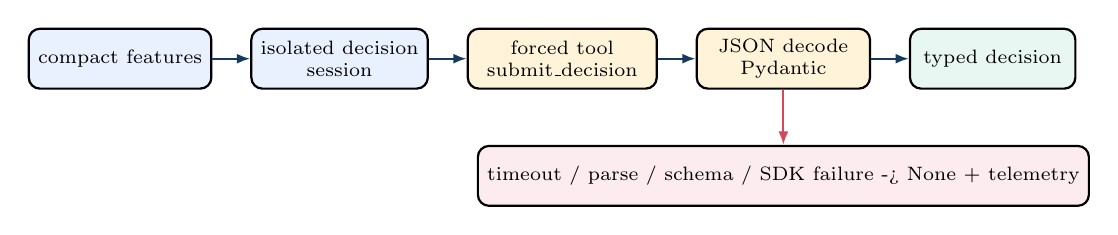
\begin{tikzpicture}[
  n/.style={draw,rounded corners,minimum height=0.76cm,align=center,font=\scriptsize,thick},
  a/.style={-{Latex[length=1.7mm]},thick,Navy},node distance=0.48cm
]
\node[n,fill=SoftBlue,minimum width=2.2cm] (features) {compact features};
\node[n,fill=SoftBlue,right=of features,minimum width=2.2cm] (session) {isolated decision\\session};
\node[n,fill=SoftAmber,right=of session,minimum width=2.4cm] (force) {forced tool\\submit\_decision};
\node[n,fill=SoftAmber,right=of force,minimum width=2.2cm] (json) {JSON decode\\Pydantic};
\node[n,fill=SoftGreen,right=of json,minimum width=2.1cm] (result) {typed decision};
\draw[a] (features)--(session);\draw[a] (session)--(force);\draw[a] (force)--(json);\draw[a] (json)--(result);
\node[n,fill=SoftRed,below=0.7cm of json,minimum width=5.2cm] (fail) {timeout / parse / schema / SDK failure -> None + telemetry};
\draw[a,Red] (json)--(fail);
\end{tikzpicture}

\vspace{0.8em}
\begin{block}{为什么这比自由文本可靠}
决策 schema 是 API 合约；失败可计数、可回放、可触发同一确定性 fallback。模型理由保留用于审计，但不能越过 Python 验证。
\end{block}
\smallsource{\pathcode{backend/intel_agent/runtime/structured.py:46-143}}
\end{frame}

\begin{frame}{本地 hooks：预算和候选约束的最后一道闸门}
\tiny
\begin{tabularx}{\textwidth}{p{0.18\textwidth} X X}
\toprule
时点 & 检查/记录 & 安全效果 \\
\midrule
PreToolUse & 总预算、每轮上限、超时、approved candidate、源/通道、重复 query & 越界在网络调用前被拒绝 \\
tool handler & 再次校验权威时间窗、参数白名单、分页、去重 & 即使 hook 漏过也不能伪造范围 \\
PostToolUse & 调用审计、结果摘要、预算计数 & reward 与 trace 有事实来源 \\
PostToolUseFailure & retryable/分页/失败原因写入 RunGap & 不把执行失败误当作语料饱和 \\
\bottomrule
\end{tabularx}

\vspace{0.2em}
\begin{alertblock}{安全模型}
\scriptsize
tool result 和 source 文本都视为不可信数据。即使其中包含 prompt injection，agent 也只有白名单工具、无 shell/文件权限，且调用参数由 handler 再验证。仍需在实验中用 AgentDojo 式恶意内容测试该假设 \cite{debenedetti2024agentdojo}。
\end{alertblock}
\smallsource{\pathcode{backend/intel_agent/hooks.py:32-178}；\pathcode{tools/source_tools.py:90-208}}
\end{frame}

\begin{frame}{故障降级格：不是一个 fallback，而是分层保底}
\small
\centering
\begin{tikzpicture}[
  level/.style={draw,rounded corners,minimum width=11.0cm,minimum height=0.65cm,align=center,font=\scriptsize,thick},
  a/.style={-{Latex[length=1.8mm]},thick,Red}
]
\node[level,fill=SoftGreen] (l1) {L1 正常：continuous SDK + approved adaptive portfolio};
\node[level,fill=SoftBlue,below=0.25cm of l1] (l2) {L2 session error：用 sdk\_session\_id resume};
\node[level,fill=SoftAmber,below=0.25cm of l2] (l3) {L3 resume 失败：fresh SDK session};
\node[level,fill=SoftRed,below=0.25cm of l3] (l4) {L4 adaptive hard failure：controller 整体降级到 legacy};
\node[level,fill=Paper,below=0.25cm of l4] (l5) {L5 持久层失败：Mongo -> JSON（若允许）并记录 error};
\draw[a] (l1)--(l2);\draw[a] (l2)--(l3);\draw[a] (l3)--(l4);\draw[a] (l4)--(l5);
\end{tikzpicture}

\vspace{0.2em}
\begin{block}{soft-complete 与 hard-failure}
SDK 报错但本轮已有 yield 可 soft-complete；没有可靠 yield 才 hard-failure。降级事件写 trace，避免静默改变实验条件。
\end{block}
\end{frame}

\begin{frame}{停止决策：adaptive 的 critic 主要解释，硬条件才决定}
\small
\begin{columns}[T,onlytextwidth]
\column{0.49\textwidth}
\begin{block}{Adaptive 权威停止原因}
\begin{enumerate}
  \item max rounds
  \item API budget exhausted
  \item timeout
  \item corpus saturated / 无可执行候选
\end{enumerate}
代码最终令 \pathcode{should_continue = (stop_reason is None)}；critic 的结构化输出用于说明与 telemetry。
\end{block}
\column{0.47\textwidth}
\begin{block}{Legacy critic + 安全阀}
优先级：max rounds $>$ stall $>$ open gaps 且有预算 $>$ min rounds。结构化 critic 失败时回到规则判断。
\end{block}
\begin{alertblock}{当前语义风险}
summary 的 \pathcode{stop_reason=null} 与 \pathcode{last_action=STOP} 可以同时出现；Control 阶段应统一终止原因 schema。
\end{alertblock}
\end{columns}
\smallsource{\pathcode{engine/controller.py:704-877}；\pathcode{agent/critic.py}}
\end{frame}

\section{核心算法与数理解释}

\begin{frame}{Legacy 覆盖：直观、便宜，但把 item 当作等质证据}
\begin{block}{默认配额}
对每个 Core 主题 $t$，相关 item 数 $n_t$ 的目标为 $q=3$：
\[
G_t^{\mathrm{legacy}}=\mathbb{1}[n_t<q],\qquad
C_t=\min\left(1,\frac{n_t}{q}\right)
\]
有 \pathcode{metadata.relevance.label} 时，只有 relevant 进入 $n_t$；无标签时按 raw score $\ge 0.5$。
\end{block}

\begin{columns}[T,onlytextwidth]
\column{0.48\textwidth}
\begin{exampleblock}{优点}
可解释、无 embedding 依赖、适合作为最小可用 fallback；stall 用连续低收益轮次识别。
\end{exampleblock}
\column{0.48\textwidth}
\begin{alertblock}{缺点}
不区分来源 trust、异源独立性、新鲜度、主题分摊和证据通道；三条同源重复边缘材料也可能“填满”。
\end{alertblock}
\end{columns}
\smallsource{\pathcode{analysis.py:26-27,63-82,179-241}；默认 stall patience=2，最低 new relevant/call=0.5。}
\end{frame}

\begin{frame}{Adaptive 覆盖目标：从一维主题计数升级为证据张量}
\begin{block}{目标集合}
\[
\mathcal{C}=\{(t,h):t\in\text{Core},\ h\in\{research,advisory\},\ \text{applicable}(t,h)\}
\]
18 个 research 单元；除 jailbreak、model backdoor 外的 16 个 advisory 单元，共 $34$ 个。
每个单元目标有效证据 $T_{t,h}=3$。
\end{block}

\centering

\begin{tikzpicture}[x=0.57cm,y=0.48cm]
\foreach \x in {0,...,17} {
  \node[draw,minimum width=0.5cm,minimum height=0.42cm,fill=SoftBlue] at (\x,1) {};
}
\foreach \x in {0,...,15} {
  \node[draw,minimum width=0.5cm,minimum height=0.42cm,fill=SoftGreen] at (\x,0) {};
}
\node[anchor=east,font=\scriptsize] at (-0.7,1) {research};
\node[anchor=east,font=\scriptsize] at (-0.7,0) {advisory};
\node[anchor=west,font=\scriptsize,text=Slate] at (18.0,1) {18 topics};
\node[anchor=west,font=\scriptsize,text=Slate] at (16.0,0) {16 applicable};
\end{tikzpicture}

\vspace{0.5em}
\begin{alertblock}{CISA exploitation 的位置}
CISA 作为确认信号进入 QueryCallOutcome/reward，但当前 \pathcode{compute_corpus_gaps} 只累积 research 与 advisory；不要声称 34 个 target 包含 exploitation。
\end{alertblock}
\smallsource{\pathcode{engine/gaps.py:51-62,147-159}}
\end{frame}

\begin{frame}{有效证据：一条 item 的贡献被五个因子共同约束}
\begin{block}{单元 $(t,h)$ 的有效证据}
\[
E_{t,h}=\sum_{i\in\mathcal I_h}
\underbrace{q_{i,t}}_{\text{topic credit}}
\underbrace{p_i}_{\text{relevance}}
\underbrace{\tau_{s(i)}}_{\text{source trust}}
\underbrace{u_i}_{\text{event uniqueness}}
\underbrace{f_{i,h}}_{\text{freshness}}
\]
\end{block}
\begin{columns}[T,onlytextwidth]
\column{0.49\textwidth}
\begin{itemize}
  \item $\sum_t q_{i,t}\le 1$：多主题 credit 守恒
  \item $p_i\in[0,1]$：irrelevant 直接置 0
  \item $\tau_s$：arXiv .72、NVD .90、OSV .84
\end{itemize}
\column{0.47\textwidth}
\begin{itemize}
  \item $u_i=1$ 首个事件，0.5 异源佐证，0 同源重复
  \item $f_{i,h}=\max(0.5,2^{-a_i/H_h})$
  \item $H_{research}=365$ 天，$H_{advisory}=730$ 天
\end{itemize}
\end{columns}
\smallsource{\pathcode{engine/gaps.py:65-176}}
\end{frame}

\begin{frame}{计算示例：两条“同事件”材料不会贡献 2 份证据}
\begin{block}{假设：同一 CVE 的首个 NVD item + 一个 OSV 异源佐证}
\[
\begin{aligned}
e_1 &= 1.0\times0.75\times0.90\times1.0\times1.0=0.675,\\
e_2 &= 1.0\times0.85\times0.84\times0.5\times1.0=0.357,\\
E &= 1.032,\qquad
G^{cov}=\max(0,1-E/3)=0.656.
\end{aligned}
\]
\end{block}

\begin{columns}[T,onlytextwidth]
\column{0.47\textwidth}
\begin{exampleblock}{得到的好处}
跨源佐证有价值，但不会与独立新事件等价；一条多标签材料也不能给每个主题都加 1。
\end{exampleblock}
\column{0.49\textwidth}
\begin{alertblock}{仍需研究}
固定 trust 与 0.5 佐证系数是工程先验，不是经验校准结果。论文实验应学习或敏感性分析这些权重。
\end{alertblock}
\end{columns}
\end{frame}

\begin{frame}{Gap 优先级：coverage 占 60\%，通道完整性和新鲜度各 20\%}
\begin{block}{三个缺口}
\[
G^{cov}_{t,h}=\max(0,1-E_{t,h}/T_{t,h}),\quad
G^{div}_{t}=1-\frac{|H^{present}_t|}{|H^{required}_t|},\quad
G^{fresh}_{t,h}=\mathbb{1}[\text{stale}]
\]
\[
P_{t,h}=\min\left(1,0.6G^{cov}_{t,h}+0.2G^{div}_{t}+0.2G^{fresh}_{t,h}\right)
\]
\end{block}

\begin{itemize}
  \item 通道在 $E_{t,h}\ge 1$ 后才算 present；fresh SLA：research 180 天、advisory 365 天。
  \item $P=0$ 才标记 satisfied；否则按 0.85/0.65/0.35 分 critical/high/medium/low。
  \item 这里的 diversity 是\alert{证据通道完整性}，不是来源数量或事件数量；命名需要在 Control 中澄清。
\end{itemize}
\smallsource{\pathcode{engine/gaps.py:180-229}}
\end{frame}

\begin{frame}{UCB 选候选：gap-aware exploitation + optimism exploration}
\scriptsize
\begin{block}{Arm}
\[
a=(topic,\ channel,\ source,\ intent,\ operator\ signature)
\]
它比“每个 source 一个 arm”更细，能区分同源不同高级算子和意图。
\end{block}
\begin{block}{当前 utility}
\[
\begin{aligned}
R_a^{exp}&=\min\left(1,0.6\sum_{g\in target(a)}P_g+0.4\max(0,\bar r_a)\right),\\
U_a&=R_a^{exp}+\sqrt{\frac{2\ln(N+2)}{n_a+1}}-0.2\,noise_a-0.2\,dup_a.
\end{aligned}
\]
\end{block}

\begin{alertblock}{理论边界}
借用了 UCB 的探索项 \cite{auer2002ucb}，但 reward 非平稳、arm 组合化、候选由 LLM 生成且有预算约束；不能直接继承经典 UCB1 regret 保证。
\end{alertblock}
\smallsource{\pathcode{engine/bandit.py:12-67}}
\end{frame}

\begin{frame}{Portfolio 与 reward：把“查到很多”改写成“减少高优先级缺口”}
\begin{columns}[T,onlytextwidth]
\column{0.48\textwidth}
\begin{block}{Portfolio 约束}
\begin{itemize}
  \item 每轮最多 4 个候选
  \item discovery 累计不超过总预算 20\%（Extended focus 可放宽）
  \item confirmation 不超过 10\%
  \item 排序确定性：utility 降序，再按 candidate ID
\end{itemize}
\end{block}
\column{0.48\textwidth}
\begin{block}{归一化 reward}
\scriptsize
\[
r=\frac{(P_{before}-P_{after})_+}{\max(1,P_{before})}
+b_{disc}+b_{conf}
-0.2\rho_{noise}-0.2\rho_{dup}-0.05
\]
最后截断到 $[-1,1]$。发现奖励最多 .25；确认奖励最多 .25。
\end{block}
\end{columns}

\begin{alertblock}{归因难点}
一个 portfolio 内多个 query 共同改变 gap；当前按调用前后优先级差归因，存在顺序效应。学术化可用 Shapley 近似、counterfactual replay 或 doubly robust estimator 改进。
\end{alertblock}
\smallsource{\pathcode{engine/bandit.py:70-127}}
\end{frame}

\begin{frame}{Checkpoint 与 RunGap：增量正确性取决于“水位能否安全推进”}
\centering
\begin{tikzpicture}[
  n/.style={draw,rounded corners,minimum height=0.72cm,minimum width=2.3cm,align=center,font=\scriptsize,thick},
  a/.style={-{Latex[length=1.7mm]},thick,Navy},node distance=0.45cm
]
\node[n,fill=SoftBlue] (scope) {checkpoint + 72h overlap\\形成权威 window};
\node[n,fill=SoftGreen,right=of scope] (call) {分页查询\\NVD/arXiv};
\node[n,fill=SoftAmber,right=of call] (proof) {success? has\_more?\\retryable?};
\node[n,fill=SoftGreen,right=of proof] (advance) {仅 success 且\\no more 时推进};
\node[n,fill=SoftRed,below=0.75cm of proof] (gap) {否则写 RunGap\\保留旧水位};
\draw[a] (scope)--(call);\draw[a] (call)--(proof);\draw[a] (proof)--(advance);\draw[a,Red] (proof)--(gap);
\end{tikzpicture}

\vspace{1em}
\begin{block}{为什么有 overlap}
数据源可能延迟发布、修改时间漂移或分页中断。72 小时重叠牺牲少量重复请求，换取不漏掉边界事件；自然键去重吸收重复。
\end{block}
\smallsource{\pathcode{engine/modes.py}；\pathcode{engine/controller.py:521-610}}
\end{frame}

\begin{frame}{新主题发现：先确定性门控，再让 LLM 命名}
\small
\begin{enumerate}
  \item residual：$p_i\ge0.7$、已知主题最大分 $<0.55$、最近 120 天；最多 500 条。
  \item embedding 聚类：任一成员余弦相似度 $\ge0.82$ 即并入。
  \item 独立性：至少 3 个 canonical events、至少 2 个 sources。
  \item 分离度：与已知 topic anchor 的最大相似度 $<0.7$。
  \item 时序：最近 30 天至少 2 个，burst ratio $\ge1.5$。
\end{enumerate}

\begin{block}{Emergence score}
\[
S=\min(1,\underbrace{\min(1,n_{event}/5)}_{support}
\underbrace{\min(1,n_{source}/3)}_{diversity}
\underbrace{\min(1,(1-s_{anchor})/0.3)}_{separation}
\underbrace{\min(1,burst/4)}_{burst}\bar p)
\]
\end{block}
只有过门控的 cluster 才交给结构化 LLM 生成名称，降低“模型凭空发明新威胁类别”的概率。
\smallsource{\pathcode{engine/gaps.py:337-447}}
\end{frame}

\begin{frame}{Playbook：跨 run 记忆的是“可复用检索技术”，不是模型自由文本}
\begin{columns}[T,onlytextwidth]
\column{0.47\textwidth}
\begin{block}{Entry}
topic bucket、source、operator signature、technique text、参数样例、reward、pulls/hits、provenance runs、embedding、status。
\end{block}
\begin{block}{召回}
有语义 query 时：相似度与 reward 加权；否则按 reward/pulls。digest 只放少量高分条目。
\end{block}
\column{0.49\textwidth}
\begin{block}{更新与衰减}
新 relevant/call $\ge0.5$ 才 harvest；未使用条目 reward $\times0.9$；pulls $\ge3$ 且 reward $<0.1$ 可 deprecated；reward $\ge1$ 且 pulls $\ge3$ 可 verified。
\end{block}
\begin{alertblock}{当前快照}
22 条：13 deprecated、8 active、1 verified。说明记忆系统已工作，但“verified”样本仍太少，暂不能证明跨 run 学习收益。
\end{alertblock}
\end{columns}
\smallsource{\pathcode{memory/playbook.py:74-239}；\pathcode{runtime_snapshot.json}}
\end{frame}

\section{持久化、可观测性与代码映射}

\begin{frame}{持久化：run 与 item 分离，去重同时保留 provenance}
\begin{columns}[T,onlytextwidth]
\column{0.49\textwidth}
\begin{block}{Mongo 主路径}
\begin{itemize}
  \item \pathcode{runs}：每个任务一份 blackboard/summary/item IDs
  \item \pathcode{items}：\pathcode{_id=item_id} 全局去重
  \item \pathcode{run_ids}：同一 item 被哪些 run 观测到
  \item \pathcode{knowledge_graphs}：item-KG 独立集合
  \item run 文档移除 raw\_text，避免重复膨胀
\end{itemize}
\end{block}
\column{0.47\textwidth}
\begin{block}{JSON fallback}
schema v3；临时文件 + 原子替换；维护 \pathcode{latest.json}；适合无 Mongo 或降级场景。
\end{block}
\begin{alertblock}{双存储口径风险}
当前 \pathcode{latest.json} 比 Mongo 最新 run 更旧。报表必须显示 storage backend 与 snapshot time，不能混合总量。
\end{alertblock}
\end{columns}
\smallsource{\pathcode{mongo_store.py:67-253}；\pathcode{persistence.py:40-103}}
\end{frame}

\begin{frame}{TraceSink：把 agent 行为变成可分析的事件流}
\scriptsize
\begin{tabularx}{\textwidth}{p{0.23\textwidth} X X}
\toprule
事件族 & 代表事件 & 可回答的问题 \\
\midrule
轮次 & round\_start, round\_summary, critic & 每轮状态、收益与停止理由如何变化？ \\
模型 & thinking, assistant\_text, session\_end & 模型花了多少 turns/cost，是否报错？ \\
工具 & tool\_call, tool\_result & 调了什么工具，参数与结果摘要是什么？ \\
恢复 & strategy\_fallback, errors & 何时改变策略，降级是否静默？ \\
UI & on\_event callback & 控制台能否实时显示同一事件？ \\
\bottomrule
\end{tabularx}

\vspace{0.2em}
\begin{alertblock}{计数口径}
\pathcode{tool_call} 包括状态、记忆、候选评分与 summary 工具；外部源 API 调用数应读取 blackboard metrics / QueryCallOutcome，不能直接使用 trace tool-call 数。
\end{alertblock}
\smallsource{\pathcode{observability.py:34-116}；\pathcode{agent/loop.py}}
\end{frame}

\begin{frame}{采集到 item-KG：清晰交接，但尚未形成全局图闭环}
\centering
\begin{tikzpicture}[
  n/.style={draw,rounded corners,minimum width=2.7cm,minimum height=0.85cm,align=center,font=\scriptsize,thick},
  a/.style={-{Latex[length=1.7mm]},thick,Navy},node distance=0.65cm
]
\node[n,fill=SoftBlue] (item) {Mongo/JSON item\\raw\_text/summary};
\node[n,fill=SoftAmber,right=of item] (elig) {eligibility + prompt\\CTINexus adapter};
\node[n,fill=SoftGreen,right=of elig] (smallkg) {item-level KG\\manifest/feedback};
\node[n,fill=Paper,right=of smallkg] (global) {未来 global KG\\schema mapping/alignment};
\draw[a] (item)-- node[above,font=\tiny]{run\_id + DTO} (elig);
\draw[a] (elig)--(smallkg);
\draw[a,dashed] (smallkg)-- node[above,font=\tiny]{尚未实现} (global);
\draw[a,dashed,bend right=28,Purple] (global.south) to node[below,font=\tiny,text=Purple]{结构 gap 反向生成 query} (item.south);
\end{tikzpicture}

\vspace{0.8em}
\begin{columns}[T,onlytextwidth]
\column{0.48\textwidth}
\begin{exampleblock}{当前验证}
smoke pipeline 通过 fake process，证明 import boundary、KG handoff 和 TraceSink 基本路径可运行。
\end{exampleblock}
\column{0.48\textwidth}
\begin{alertblock}{尚未完成}
item-KG 与 base KG 的 schema mapping、实体对齐、冲突合并、provenance confidence 和质量门控仍是路线图。
\end{alertblock}
\end{columns}
\smallsource{CTINexus 方法参照 \cite{cheng2025ctinexus}；CTI 互操作参照 STIX 2.1 \cite{stix21}}
\end{frame}

\begin{frame}{代码地图：从报告概念回到当前实现}
\scriptsize
\begin{tabularx}{\textwidth}{p{0.20\textwidth} p{0.36\textwidth} X}
\toprule
概念 & 主要文件 & 权威职责 \\
\midrule
taxonomy & \pathcode{backend/common/topics.py} & Core/Extended、关键词、anchors \\
状态/schema & \pathcode{backend/intel_agent/schemas.py} & item、candidate、gap、checkpoint、blackboard \\
控制器 & \pathcode{engine/controller.py} & 模式边界、轮次、fallback、stop、persist \\
覆盖/发现 & \pathcode{engine/gaps.py} & 有效证据、priority、trend、emergence \\
bandit & \pathcode{engine/bandit.py} & arm、UCB、portfolio、reward \\
相关性 & \pathcode{relevance.py} & rule/embedding/LLM、cache \\
数据源 & \pathcode{sources.py} & HTTP、operator、parser、初始 score \\
工具/约束 & \pathcode{tools/*.py}, \pathcode{hooks.py} & MCP 白名单、候选与预算校验 \\
SDK & \pathcode{agent/loop.py}, \pathcode{runtime/*.py} & session、tool-forcing、provider、恢复 \\
存储/观测 & \pathcode{mongo_store.py}, \pathcode{persistence.py}, \pathcode{observability.py} & provenance、原子写、JSONL trace \\
下游 KG & \pathcode{backend/ctinexus_kg/} & item 级构图，失败隔离 \\
\bottomrule
\end{tabularx}
\end{frame}

\begin{frame}{源码审计发现的五个“容易误读”点}
\begin{enumerate}
  \item \risk\ full 可使用 SDK，但\alert{不是} adaptive CorpusGap 路径。
  \item \risk\ \pathcode{core_gap_count=0} 可能只是 CorpusGap 列表为空；不代表 legacy 配额已满足。
  \item \risk\ \pathcode{stop_reason=null} 可与最后动作 STOP 并存，终止 schema 不一致。
  \item \risk\ \pathcode{INTEL_ENGINE=rules} 仍留在部分环境文档，但当前 controller/CLI 主路径不读取它。
  \item \risk\ adaptive MCP 不暴露 \pathcode{record_technique}，但 controller 会根据真实 outcome 自动 harvest；不能只看 prompt 判断记忆是否写入。
\end{enumerate}

\vspace{0.7em}
\begin{block}{审计结论}
这类差异不会让系统“不能跑”，但会让实验分组、看板和论文叙述失真。DMAIC 的 Control 必须把这些语义写成数据契约测试。
\end{block}
\end{frame}

\section{真实运行结果与诊断}

\begin{frame}{验证基线：当前工作树的规定测试与冒烟均通过}
\centering
\metric{86}{passed}\hfill
\metric{0}{failed}\hfill
\metric{10.09 s}{pytest}\hfill
\metric{PASS}{smoke pipeline}

\vspace{1.2em}
\begin{block}{执行命令}
\small\ttfamily
uv run pytest backend/intel\_agent/tests backend/ctinexus\_kg/tests backend/console/tests -q

uv run python scripts/smoke\_pipeline.py
\end{block}

\begin{columns}[T,onlytextwidth]
\column{0.48\textwidth}
\begin{exampleblock}{测试证明了什么}
schema、算法、fallback、工具约束、存储、UI 组件及 fake KG 交接的已编码不变量没有回归。
\end{exampleblock}
\column{0.48\textwidth}
\begin{alertblock}{没有证明什么}
真实外部源 recall、人工 precision、跨 provider 稳定性、长时 full campaign、恶意内容安全和全局 KG 质量。
\end{alertblock}
\end{columns}
\end{frame}

\begin{frame}{Mongo 历史：规模已形成，但来源高度偏向 arXiv}
\begin{columns}[T,onlytextwidth]
\column{0.62\textwidth}
\begin{tikzpicture}
\begin{axis}[
  xbar,
  width=8.0cm,height=5.2cm,
  xmin=0,xmax=5800,
  symbolic y coords={CISA,OSV,NVD,arXiv},
  ytick=data,
  xlabel={全局去重 items},
  nodes near coords,
  nodes near coords align={horizontal},
  bar width=10pt,
  axis line style={draw=Slate},
  tick label style={font=\scriptsize},
  label style={font=\scriptsize},
  enlarge y limits=0.15
]
\addplot[fill=Blue,draw=Blue] coordinates {(268,CISA) (536,OSV) (936,NVD) (5209,arXiv)};
\end{axis}
\end{tikzpicture}
\column{0.34\textwidth}
\begin{block}{统一快照}
\begin{itemize}
  \item 12 runs
  \item 6,949 distinct items
  \item 2,505 items 跨 run 重现
  \item 3 item-KGs
\end{itemize}
\end{block}
\begin{alertblock}{来源占比}
arXiv 75.0\%；NVD 13.5\%；OSV 7.7\%；CISA 3.9\%。高吞吐 research 通道主导 corpus。
\end{alertblock}
\end{columns}
\smallsource{Mongo \pathcode{intel_agent}，2026-07-15 12:48 UTC；\pathcode{runtime_snapshot.json}}
\end{frame}

\begin{frame}{主题分布：头部充足，部分 Core 几乎没有证据}
\small
\begin{columns}[T,onlytextwidth]
\column{0.58\textwidth}
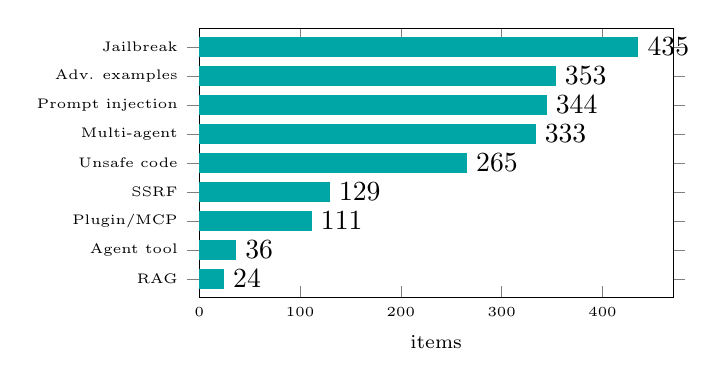
\begin{tikzpicture}
\begin{axis}[
  xbar,width=7.6cm,height=5.0cm,
  xmin=0,xmax=470,
  symbolic y coords={RAG,Agent tool,Plugin/MCP,SSRF,Unsafe code,Multi-agent,Prompt injection,Adv. examples,Jailbreak},
  ytick=data,nodes near coords,bar width=7pt,
  tick label style={font=\tiny},label style={font=\scriptsize},
  xlabel={items},enlarge y limits=0.08
]
\addplot[fill=Cyan,draw=Cyan] coordinates {
  (24,RAG) (36,Agent tool) (111,Plugin/MCP) (129,SSRF) (265,Unsafe code)
  (333,Multi-agent) (344,Prompt injection) (353,Adv. examples) (435,Jailbreak)};
\end{axis}
\end{tikzpicture}
\column{0.38\textwidth}
\begin{alertblock}{弱覆盖主题}
\scriptsize
\begin{tabular}{lr}
excessive agency & 6\\
unbounded consumption & 6\\
insecure output handling & 4\\
model denial of service & 2\\
logging/monitoring & 1\\
misinformation/citation & 1\\
internal recon & 1\\
\end{tabular}
\end{alertblock}
\begin{block}{不能仅看 count}
这些是主题标签 item 数，不等于独立事件数或有效证据；但长尾足以说明固定查询策略存在结构性盲点。
\end{block}
\end{columns}
\end{frame}

\begin{frame}{相关性测量：67.4\% 为 uncertain，LLM 复核仅占 0.35\%}
\small
\begin{columns}[T,onlytextwidth]
\column{0.46\textwidth}
\begin{block}{标签分布（6,949）}
\begin{tabularx}{0.96\linewidth}{X r r}
\toprule
label & count & share \\
\midrule
uncertain & 4,683 & 67.39\% \\
relevant & 2,157 & 31.04\% \\
irrelevant & 109 & 1.57\% \\
\bottomrule
\end{tabularx}
\end{block}
\column{0.46\textwidth}
\begin{block}{决策方法}
\begin{tabularx}{0.96\linewidth}{X r r}
\toprule
method & count & share \\
\midrule
rule & 5,976 & 86.00\% \\
embedding & 949 & 13.66\% \\
LLM & 24 & 0.35\% \\
\bottomrule
\end{tabularx}
\end{block}
\end{columns}

\begin{alertblock}{诊断}
系统不是“缺少分类结果”，而是大量样本落在灰区。下一步不是简单放宽阈值，而是抽样标注、校准 score、核对 escalation 配置和 LLM batch 实际触发率。
\end{alertblock}
\end{frame}

\begin{frame}{最新 full/bootstrap：能正常停止，但覆盖结构明显不足}
\centering
\metric{3}{rounds}\hfill
\metric{12}{source API calls}\hfill
\metric{28}{items}\hfill
\metric{229.7 s}{elapsed}

\vspace{0.9em}
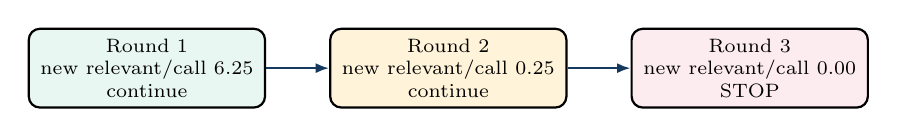
\begin{tikzpicture}[
  n/.style={draw,rounded corners,minimum width=3.0cm,minimum height=1.0cm,align=center,font=\scriptsize,thick},
  a/.style={-{Latex[length=1.7mm]},thick,Navy}
]
\node[n,fill=SoftGreen] (r1) {Round 1\\new relevant/call 6.25\\continue};
\node[n,fill=SoftAmber,right=0.8cm of r1] (r2) {Round 2\\new relevant/call 0.25\\continue};
\node[n,fill=SoftRed,right=0.8cm of r2] (r3) {Round 3\\new relevant/call 0.00\\STOP};
\draw[a] (r1)--(r2);\draw[a] (r2)--(r3);
\end{tikzpicture}

\vspace{0.7em}
\begin{columns}[T,onlytextwidth]
\column{0.47\textwidth}
\begin{block}{事实}
28 条全部来自 NVD；仅使用 1 个 source；15/18 Core legacy 配额仍未满足；最后动作 STOP。
\end{block}
\column{0.49\textwidth}
\begin{alertblock}{schema 反例}
summary 同时给出 \pathcode{core_gap_count=0}、15 个 \pathcode{coverage_gaps_remaining}、\pathcode{stop_reason=null}。前者不能被用作“覆盖完成”。
\end{alertblock}
\end{columns}
\smallsource{run \pathcode{real-intel-agent-bootstrap-20260715T120801Z}}
\end{frame}

\begin{frame}{最新 trace：137 个事件可回放，SDK 成本约 0.475 美元}
\begin{columns}[T,onlytextwidth]
\column{0.57\textwidth}
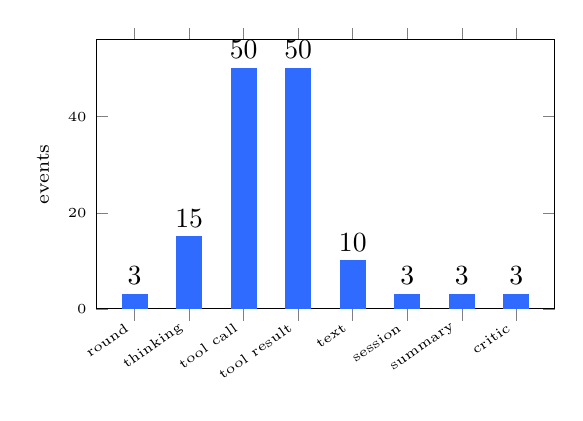
\begin{tikzpicture}
\begin{axis}[
  ybar,width=7.4cm,height=5.0cm,ymin=0,ymax=56,
  symbolic x coords={round,thinking,tool call,tool result,text,session,summary,critic},
  xtick=data,xticklabel style={rotate=35,anchor=east,font=\tiny},
  nodes near coords,bar width=9pt,
  tick label style={font=\tiny},label style={font=\scriptsize},ylabel={events}
]
\addplot[fill=Blue,draw=Blue] coordinates {(round,3) (thinking,15) (tool call,50) (tool result,50) (text,10) (session,3) (summary,3) (critic,3)};
\end{axis}
\end{tikzpicture}
\column{0.39\textwidth}
\begin{block}{Session 汇总}
\begin{itemize}
  \item SDK turns：53
  \item cost：\$0.47506
  \item session errors：0
  \item trace file：同 run ID JSONL
\end{itemize}
\end{block}
\begin{alertblock}{不要相除}
50 个 tool calls 并非 50 个源请求；blackboard 的源 API calls 是 12。
\end{alertblock}
\end{columns}
\end{frame}

\begin{frame}{根因链：最新结果不是单点故障，而是路径与目标不一致}
\centering
\begin{tikzpicture}[
  n/.style={draw,rounded corners,minimum width=2.4cm,minimum height=0.8cm,align=center,font=\scriptsize,thick},
  a/.style={-{Latex[length=1.7mm]},thick,Red},node distance=0.42cm
]
\node[n,fill=SoftRed] (goal) {用户目标：完整\\LLM 安全初始语料};
\node[n,fill=SoftAmber,right=of goal] (mode) {选择 full\\但 full=legacy quota};
\node[n,fill=SoftAmber,right=of mode] (query) {本轮策略集中 NVD\\无 source diversity};
\node[n,fill=SoftAmber,right=of query] (stop) {边际 yield 下降\\critic STOP};
\node[n,fill=SoftRed,right=of stop] (out) {28 items\\15 gap 未满足};
\draw[a] (goal)--(mode);\draw[a] (mode)--(query);\draw[a] (query)--(stop);\draw[a] (stop)--(out);
\end{tikzpicture}

\vspace{1em}
\begin{block}{Why-Why 结论}
停止本身符合 legacy 低收益规则；真正的问题是 full 的 measurement/coverage contract 没有表达“每个主题需要哪些证据通道、多少独立事件、何种新鲜度”，所以 controller 无法把业务目标转成可验证终态。
\end{block}
\end{frame}

\begin{frame}{运行结论：可用性不是“能跑”，而是稳定交付满足合同的 corpus}
\begin{columns}[T,onlytextwidth]
\column{0.48\textwidth}
\begin{exampleblock}{当前可称为成熟的部分}
\begin{itemize}
  \item 软件边界与测试基线
  \item 多源连接、解析、去重与持久化
  \item SDK 白名单、hook、trace、fallback
  \item adaptive 算法组件已编码
\end{itemize}
\end{exampleblock}
\column{0.48\textwidth}
\begin{alertblock}{尚不能宣称成熟的部分}
\begin{itemize}
  \item full/bootstrap 的有效覆盖与可恢复性
  \item relevance/topic measurement validity
  \item 同预算下 adaptive 的增益与统计显著性
  \item 新主题真实 precision
  \item item-KG 到 global KG 的质量闭环
\end{itemize}
\end{alertblock}
\end{columns}

\vspace{0.5em}
\begin{center}
\Large 北极星：\textcolor{Purple}{固定预算下，交付质量验证、结构覆盖、可恢复且可追溯的初始语料库}
\end{center}
\end{frame}

\section{学术综述与研究空白}

\begin{frame}{综述协议：范围综述，不伪装成 PRISMA 系统综述}
\scriptsize
\begin{columns}[T,onlytextwidth]
\column{0.48\textwidth}
\begin{block}{检索与纳入}
\begin{itemize}
  \item 截止：2026-07-15
  \item arXiv/作者页、OpenReview、IEEE/DOI
  \item NIST、OWASP、MITRE、OASIS 与源官方文档
  \item 纳入原始研究、正式标准、官方数据文档
  \item 预印本显式标注；排除产品宣传与不可核验二手材料
\end{itemize}
\end{block}
\column{0.48\textwidth}
\begin{block}{四条研究流}
\begin{enumerate}
  \item agent reasoning/tool use/evaluation
  \item active search/bandit/closed-loop control
  \item LLM/agent security taxonomy and benchmarks
  \item CTI collection, standards and knowledge graphs
\end{enumerate}
最终保留 20 个核心来源。
\end{block}
\end{columns}
\smallsource{完整检索词、矩阵与注释书目：\pathcode{report/literature_review.md}}
\end{frame}

\begin{frame}{综述证据边界：新兴 agent 研究与成熟基础理论分开解读}
\small
\begin{columns}[T,onlytextwidth]
\column{0.48\textwidth}
\begin{block}{时间结构}
2024--2026 工作占比较高，反映 agentic search 与 agent security 的快速演进；同时保留 2002/2003/2012 的 UCB、MAPE-K 与 active search 基础工作，避免把“新”误当“已验证”。
\end{block}
\column{0.48\textwidth}
\begin{block}{证据等级}
正式论文/标准用于方法与定义；预印本用于识别前沿方向；官方 API 文档只证明源能力，不证明算法效果。所有性能主张最终都要由本项目冻结 benchmark 与人工 gold 重测。
\end{block}
\end{columns}

\begin{alertblock}{范围限制}
本综述服务于系统定位和实验设计，不声称完成数据库穷尽检索、双人筛选或发表偏倚评估；因此称为范围综述，而非 PRISMA 系统综述。
\end{alertblock}
\end{frame}

\begin{frame}{研究版图：四条成熟链条尚未在一个系统中闭环}
\scriptsize
\begin{tabularx}{\textwidth}{p{0.17\textwidth} p{0.23\textwidth} X X}
\toprule
研究流 & 代表工作 & 已解决 & 对本项目留下的空白 \\
\midrule
Agent & ReAct、AgentBench、AgentDojo & 推理-行动闭环、多环境能力、utility/security 同测 & 异质 CTI 来源、覆盖合同、可恢复 campaign \\
Search & Search-R1、active search、UCB & 多轮 query、固定预算发现、探索/利用 & source applicability、非平稳 reward、证据独立性 \\
Security & OWASP、MITRE ATLAS、NIST RMF & 风险分类、攻击技术、治理/TEVV & 可计算 topic-channel target 与运行级 stop risk \\
CTI/KG & STIX、CTINexus、AttacKG+、KnowCTI、ThreatKG & 标准表达、抽取、实体对齐、攻击图 & 上游主动采集与 KG gap 反向查询 \\
\bottomrule
\end{tabularx}

\vspace{0.7em}
\begin{center}
\textcolor{Purple}{论文机会 = 把四条链的“接口缺口”形式化并实验验证，而不是再做一个通用 agent 框架。}
\end{center}
\end{frame}

\begin{frame}{Agentic search 文献：重点从“会调用工具”转向“如何评价过程”}
\small
\begin{columns}[T,onlytextwidth]
\column{0.49\textwidth}
\begin{block}{方法脉络}
\begin{itemize}
  \item ReAct：reasoning/action 交错，环境反馈修正计划 \cite{yao2023react}
  \item Search-R1：用结果 reward 学习多轮 search，而非只在推理时提示 \cite{jin2025searchr1}
  \item Active Search：固定预算最大化发现目标类的数量 \cite{garnett2012active}
  \item UCB：在未知收益 arm 间平衡探索与利用 \cite{auer2002ucb}
\end{itemize}
\end{block}
\column{0.47\textwidth}
\begin{block}{评测脉络}
\begin{itemize}
  \item AgentBench：8 个交互环境，暴露长期推理/决策问题 \cite{liu2024agentbench}
  \item DeepResearch Bench：100 任务、22 学科；评价有效引用和引用准确率 \cite{du2025deepresearchbench}
  \item AgentDojo：97 任务、629 安全用例，同测 utility 与 prompt injection \cite{debenedetti2024agentdojo}
\end{itemize}
\end{block}
\end{columns}

\begin{alertblock}{转化到本项目}
最终 item 质量、过程 trace、来源引用、策略安全和预算效率必须一起评价；单一 final answer 或 item count 不足以说明 agent 可用。
\end{alertblock}
\end{frame}

\begin{frame}{CTI 与安全文献：结构化能力成熟，上游获取仍是开放问题}
\small
\begin{columns}[T,onlytextwidth]
\column{0.48\textwidth}
\begin{block}{风险与标准}
\begin{itemize}
  \item OWASP 2025：应用级十大 LLM 风险 \cite{owaspllm2025}
  \item MITRE ATLAS：AI tactic/technique/mitigation/case studies \cite{mitreatlas}
  \item NIST AI RMF/GAI Profile：Govern/Map/Measure/Manage 与 TEVV \cite{nistairmf2023,nistgai2024}
  \item STIX 2.1：CTI 对象关系与交换 \cite{stix21}
\end{itemize}
\end{block}
\column{0.48\textwidth}
\begin{block}{知识图谱}
\begin{itemize}
  \item CTINexus：ICL、层次实体对齐、长关系补全，150 报告/10 平台 \cite{cheng2025ctinexus}
  \item AttacKG+：时间展开攻击图 + TTP \cite{zhang2024attackgkplus}
  \item KnowCTI：领域知识增强实体/关系抽取 \cite{knowcti2024}
  \item ThreatKG：多源 OSCTI 持续采集与入图 \cite{threatkg2022}
\end{itemize}
\end{block}
\end{columns}

\begin{alertblock}{共同缺口}
这些工作多数优化“文档到图”的质量；很少用图的结构空洞、不确定边和 provenance 冲突反向决定下一轮去哪个源、查什么、何时停止。
\end{alertblock}
\end{frame}

\begin{frame}{研究空白 -> 可检验贡献}
\scriptsize
\begin{tabularx}{\textwidth}{p{0.26\textwidth} X X}
\toprule
空白 & 本项目可贡献 & 可验证证据 \\
\midrule
结构化覆盖缺口 & topic-channel-quality evidence tensor & 人工标注 benchmark 上 coverage/precision \\
跨源 reward 不可比 & source-aware contextual/constraint bandit & 同预算 A/B + regret/reward calibration \\
停止无风险语义 & confidence/risk-bounded stopping & premature-stop 与 waste 分解 \\
测量误差被忽略 & relevance/topic/event MSA + uncertainty propagation & 双标注、Kappa、ECE、bootstrap CI \\
采集与 KG 单向 & KG-gap-driven query generation & 图完整度、冲突率、下游问答/调查任务 \\
缺少公开过程数据 & trace-level LLM-security CTI benchmark & 任务、快照、mock API、seed、成本清单 \\
\bottomrule
\end{tabularx}

\end{frame}

\begin{frame}{研究定位：把四条链的接口缺口变成一篇可证伪论文}
\begin{center}
\Large\textcolor{Purple}{\textbf{EvidenceGap-Agent}}\\[0.4em]
\large Risk-bounded Active Intelligence Collection for LLM Security
\end{center}

\vspace{0.8em}
\begin{columns}[T,onlytextwidth]
\column{0.48\textwidth}
\begin{block}{论文核心}
用质量加权的有效证据状态表示“还缺什么”，以 source-aware 策略主动查询，并在覆盖、精度、风险与预算约束下停止。
\end{block}
\column{0.48\textwidth}
\begin{block}{区别于通用 agent}
贡献不依赖更大的模型，而来自问题形式化、证据张量、约束策略、停止条件、过程 benchmark 与可复现实证。
\end{block}
\end{columns}

\begin{alertblock}{最重要的审稿问题}
新指标是否真的对应分析师价值？新策略是否在同预算、同源快照、强基线和人工 gold 上显著优于当前实现？
\end{alertblock}
\end{frame}

\section{完整 DMAIC 可用性提升设计}

\begin{frame}{DMAIC 总览：先修测量，再调策略，最后固化控制}
\centering
\resizebox{0.96\linewidth}{!}{%
\begin{tikzpicture}[
  phase/.style={draw,rounded corners=3pt,minimum width=2.35cm,minimum height=1.15cm,align=center,font=\small\bfseries,thick},
  a/.style={-{Latex[length=2mm]},thick,Navy},node distance=0.35cm
]
\node[phase,fill=SoftBlue] (d) {D - Define\\覆盖合同/用户价值};
\node[phase,fill=SoftGreen,right=of d] (m) {M - Measure\\MSA/基线/数据计划};
\node[phase,fill=SoftAmber,right=of m] (a1) {A - Analyze\\根因/假设/优先级};
\node[phase,fill=SoftRed,right=of a1] (i) {I - Improve\\实验/实现/试点};
\node[phase,fill=Paper,right=of i] (c) {C - Control\\SPC/回滚/治理};
\draw[a] (d)--(m);\draw[a] (m)--(a1);\draw[a] (a1)--(i);\draw[a] (i)--(c);
\end{tikzpicture}
}

\vspace{1em}
\begin{tabularx}{\textwidth}{p{0.14\textwidth} X X}
\toprule
Tollgate & 必须交付 & 放行条件 \\
\midrule
D & charter、SIPOC、VOC-CTQ、范围与风险 & “可用 corpus”定义无歧义 \\
M & 冻结 benchmark、操作定义、MSA、现状能力 & 标签/事件/主题测量达到门槛 \\
A & Pareto、因果图、验证过的根因 & 至少一条证据支持每个优先根因 \\
I & DOE/A-B、pilot、FMEA、变更包 & 主要 CTQ 改善且无安全/成本回退 \\
C & control plan、看板、告警、回滚与审计 & 连续 4 周/多个 campaign 稳定 \\
\bottomrule
\end{tabularx}
\end{frame}

\begin{frame}{Define 1：项目章程与问题陈述}
\begin{columns}[T,onlytextwidth]
\column{0.49\textwidth}
\begin{block}{Problem statement}
当前系统能稳定采集与持久化，但 latest full 仅从 NVD 获得 28 条、15 个 Core quota gap 未满足；全库 67.4\% uncertain、75.0\% 来自 arXiv。现有 full 终态不能证明 corpus 的质量、证据结构或可恢复性。
\end{block}
\begin{block}{Business case}
降低人工检索与复核成本；更快发现 LLM/agent 风险；给 item-KG/global KG 提供可追溯、结构平衡的输入。
\end{block}
\column{0.47\textwidth}
\begin{block}{Goal statement（建议）}
在冻结预算与源快照上，将 quality-validated weighted coverage 提升到 $\ge0.90$，无 critical gap；人工 precision $\ge0.85$；uncertain $\le0.25$；100\% campaign 可恢复；单位有效证据成本不高于基线 1.25 倍。
\end{block}
\begin{block}{Scope}
In：intel\_agent full/incremental、四源、relevance、Mongo/trace、item-KG handoff。Out：base KG 本体重构、生产 SOC 响应、全自动漏洞处置。
\end{block}
\end{columns}
\end{frame}

\begin{frame}{Define 2：VOC -> CTQ 与 SIPOC}
\scriptsize
\begin{tabularx}{\textwidth}{p{0.15\textwidth} p{0.23\textwidth} X p{0.22\textwidth}}
\toprule
Voice & 需要 & CTQ & 缺陷定义 \\
\midrule
安全分析师 & 少噪声、可追溯、可复核 & precision、provenance completeness & 无法证实来源或错误相关 \\
研究人员 & 主题与研究/漏洞证据都覆盖 & weighted evidence coverage、independence & critical cell 未满足 \\
运维 & 可控成本、可恢复、失败不静默 & cost/evidence、resume success、fallback visibility & 丢水位/静默降级/超预算 \\
KG 消费方 & DTO 完整、实体锚点、文本质量 & handoff completeness、ID density & 缺 raw/summary/source/ID \\
治理方 & 安全工具使用、版本可审计 & policy violation rate、trace completeness & 越权调用或 trace 缺失 \\
\bottomrule
\end{tabularx}

\vspace{0.5em}
\begin{block}{SIPOC}
\textbf{Suppliers}: NVD/CISA/OSV/arXiv、LLM provider、taxonomy owner
$\rightarrow$ \textbf{Inputs}: API records、goal、budget、checkpoint、playbook
$\rightarrow$ \textbf{Process}: plan-call-parse-relevance-gap-stop-persist
$\rightarrow$ \textbf{Outputs}: corpus、gap state、trace、item-KG queue
$\rightarrow$ \textbf{Customers}: analyst、researcher、KG、console/ops。
\end{block}
\end{frame}

\begin{frame}{Measure 1：指标操作定义 - 避免同名异义}
\scriptsize
\begin{tabularx}{\textwidth}{p{0.22\textwidth} X p{0.24\textwidth}}
\toprule
CTQ & 计算定义 & 数据源/频率 \\
\midrule
人工 precision & 双标注 relevant / 被系统判 relevant & 每版本分层抽样 \\
Recall proxy & 冻结 gold events 中被自然键或人工语义匹配召回的比例 & 每次 benchmark \\
Weighted coverage & $1-\sum w_gG^{cov}_g/\sum w_g$；另报 critical gap count & 每 run/每轮 \\
Independent evidence & canonical events / relevant items；异源佐证另报 & 每 run \\
Freshness compliance & 有效证据最新时间满足 channel SLA 的 cell 比例 & 每日 \\
Efficiency & $\Delta$ effective evidence / source API call；并报美元与秒 & 每轮/每 run \\
Handoff completeness & 必需 DTO 字段完整且可入 KG queue 的 item 比例 & 每 run \\
Resumability & 注入中断后无遗漏/无水位跳跃完成的 campaign 比例 & 每发布 \\
Safety & 越权 tool call、未审计 fallback、恶意内容导致违规动作的比例 & 每安全套件 \\
\bottomrule
\end{tabularx}
\end{frame}

\begin{frame}{Measure 2：MSA - relevance、topic 与 event 三套量具分别验证}
\scriptsize
\begin{columns}[T,onlytextwidth]
\column{0.49\textwidth}
\begin{block}{抽样设计}
\begin{itemize}
  \item $n=600$，按 4 sources × 初判标签 × 时间层分层
  \item 2 名安全标注员独立判断；冲突由第 3 人裁决
  \item 14 天后对 15\% 样本重复标注，测 repeatability
  \item 保留 title/summary/raw/source，不显示系统 score 以减少锚定
\end{itemize}
\end{block}
\column{0.47\textwidth}
\begin{block}{量具与门槛（建议）}
\begin{itemize}
  \item relevance：Cohen $\kappa\ge0.75$
  \item multi-label topic：macro F1 $\ge0.80$，Jaccard $\ge0.75$
  \item canonical event：pair agreement $\ge0.95$
  \item score calibration：ECE $\le0.05$，Brier score 报告 CI
  \item 若不达标：修订 rubric/anchor，再测，不进入 Analyze
\end{itemize}
\end{block}
\end{columns}

\begin{alertblock}{关键纪律}
uncertain 不计作健康覆盖。若业务允许软证据，必须以校准后的概率和置信区间传播，而不是把标签名称直接变成常数权重。
\end{alertblock}
\end{frame}

\begin{frame}{Measure 3：基线数据计划与分层}
\scriptsize
\begin{tabularx}{\textwidth}{p{0.18\textwidth} X X}
\toprule
数据集 & 设计 & 目的 \\
\midrule
Frozen-source replay & 保存源响应/时间戳/分页，30 个任务 × 5 seeds & 消除 live source 漂移，比较算法 \\
Live shadow & 同一天、同预算交错运行策略，不自动入主库 & 验证外部有效性与时延/限流 \\
Adversarial source & 注入 prompt、伪 CVE、重复事件、污染 metadata & 验证 hooks、parser、relevance、安全 \\
Interruption suite & 在分页、persist、SDK session、Mongo 处注入故障 & 验证 checkpoint/resume/fallback \\
Human gold & 600 MSA + 每任务事件/主题 gold 子集 & precision、recall proxy、calibration \\
KG handoff & 固定 100 item，含空 raw、同义实体、冲突 provenance & DTO 完整与下游质量 \\
\bottomrule
\end{tabularx}

\vspace{0.2em}
\begin{block}{分层原则}
所有指标按 source、topic rarity、channel、query intent、provider、fallback state、time window 分层；总均值只作摘要，不能掩盖长尾主题和单源失败。
\end{block}
\end{frame}

\begin{frame}{Analyze 1：当前证据支持的因果假设}
\small
\begin{tabularx}{\textwidth}{p{0.28\textwidth} X p{0.22\textwidth}}
\toprule
假设 & 现有证据 & 下一步验证 \\
\midrule
H-A1 full 目标函数错位 & full 条件在 controller 明确排除 adaptive；latest 有 15 quota gap 且 0 CorpusGap & 同预算 legacy vs campaign \\
H-A2 relevance 量具失真 & uncertain 67.4\%；LLM 判定仅 0.35\%；raw score 从 .45 起 & MSA + threshold/calibration \\
H-A3 吞吐 reward 引起 source skew & arXiv 占 75.0\%；高吞吐源天然赢 new-items/call & source-normalized reward 消融 \\
H-A4 stop 缺乏交付合同 & last action STOP 与 stop\_reason null；未满足 gap 仍停 & risk-bounded stop A/B \\
H-A5 schema/看板语义导致误判 & core\_gap\_count=0 与 15 legacy gaps 并存 & contract tests + dashboard audit \\
H-A6 playbook 学习信号稀疏 & 22 条中仅 1 verified、13 deprecated & replay with/without memory \\
\bottomrule
\end{tabularx}
\end{frame}

\begin{frame}{Analyze 2：Pareto + FMEA，而不是凭直觉排期}
\begin{columns}[T,onlytextwidth]
\column{0.47\textwidth}
\begin{block}{缺陷 Pareto 建议分类}
\begin{enumerate}
  \item false relevant / uncertain overflow
  \item critical cell uncovered
  \item source/channel imbalance
  \item premature stop / budget waste
  \item checkpoint or persistence gap
  \item missing provenance / KG handoff defect
  \item policy violation / silent fallback
\end{enumerate}
按对 CTQ 的损失而非事件次数排序。
\end{block}
\column{0.49\textwidth}
\begin{block}{FMEA 评分}
对 failure mode 评 Severity $S$、Occurrence $O$、Detection $D$，$RPN=SOD$；另强制将任何越权工具调用、checkpoint 跳跃、provenance 丢失设为 stop-ship，不允许被低频稀释。
\end{block}
\begin{alertblock}{因果验证}
使用冻结 replay 改一个因子；live shadow 做外部验证。相关性只说明线索，不等于根因。
\end{alertblock}
\end{columns}
\end{frame}

\begin{frame}{Improve 1：五个改进包与优先顺序}
\scriptsize
\begin{tabularx}{\textwidth}{p{0.11\textwidth} p{0.22\textwidth} X p{0.18\textwidth}}
\toprule
优先级 & 改进包 & 具体动作 & 成功门槛 \\
\midrule
P0 & Measurement contract & MSA、probability calibration、统一 stop/gap schema、data contract tests & 量具门槛全通过 \\
P1 & Full campaign & full 复用 CorpusGap/UCB/checkpoint；阶段化 seed-gap-confirm-discover-handoff；可 resume & coverage $\ge.90$，无 critical \\
P2 & Source-aware policy & applicability mask、cost/latency normalized contextual bandit、portfolio attribution & 同预算 evidence/call 提升 \\
P3 & Active relevance & uncertainty sampling、source/topic calibration、LLM escalation budget、hard negatives & uncertain $\le.25$，precision $\ge.85$ \\
P4 & KG closed loop & schema mapping、entity alignment、conflict/provenance、KG gap -> query & 图完整度/下游任务提升 \\
\bottomrule
\end{tabularx}

\vspace{0.6em}
\begin{alertblock}{发布原则}
每个改进包先 frozen replay，再 shadow，最后 5\% canary；任何 safety、precision 或 resumability stop-ship 指标回退即自动 rollback。
\end{alertblock}
\end{frame}

\begin{frame}{Improve 2：把 full 重构为可恢复的阶段化 Bootstrap Campaign}
\centering
\begin{tikzpicture}[
  n/.style={draw,rounded corners,minimum width=2.25cm,minimum height=0.9cm,align=center,font=\scriptsize\bfseries,thick},
  a/.style={-{Latex[length=1.7mm]},thick,Navy},node distance=0.35cm
]
\node[n,fill=SoftBlue] (seed) {1 Seed sweep\\适用源最小探测};
\node[n,fill=SoftGreen,right=of seed] (gap) {2 Gap fill\\高 P cell};
\node[n,fill=SoftAmber,right=of gap] (confirm) {3 Confirm\\CISA/异源佐证};
\node[n,fill=SoftRed,right=of confirm] (discover) {4 Discover\\Extended/residual};
\node[n,fill=Paper,right=of discover] (handoff) {5 Handoff\\质量清单/manifest};
\draw[a] (seed)--(gap);\draw[a] (gap)--(confirm);\draw[a] (confirm)--(discover);\draw[a] (discover)--(handoff);
\draw[a,dashed,bend left=30] (discover.north) to node[above,font=\tiny]{新 candidate 经审批进入 taxonomy backlog} (gap.north);
\end{tikzpicture}

\vspace{0.8em}
\begin{block}{Campaign stop contract}
只有同时满足：no critical gap；weighted coverage 达标；precision 下置信界达标；checkpoint/run gaps 清零或显式 waiver；预算/成本在界内；manifest 与 trace 完整，才可标记 complete。
\end{block}

\begin{block}{可恢复状态}
每个阶段、cell、candidate、source page、watermark、failure、model/prompt/taxonomy version 都持久化；重启从最后 confirmed checkpoint 继续，而非重新“full”。
\end{block}
\end{frame}

\begin{frame}{Control：Control Plan、SPC、告警与反应规则}
\scriptsize
\begin{tabularx}{\textwidth}{p{0.18\textwidth} p{0.18\textwidth} p{0.17\textwidth} X}
\toprule
指标 & 图/频率 & 触发条件 & 反应计划 \\
\midrule
人工 precision & p-chart / 每周样本 & LCL 低于 .85 或连续 2 点下行 & 停止自动入库，回滚阈值/模型，复核最近批次 \\
uncertain share & p-chart / 每 run & $> .25$ 或 source 单层异常 & 检查 embedding/LLM escalation、漂移样本 \\
weighted coverage & run chart / 每轮 & critical gap 两轮不降 & 重排 portfolio，打开专家 review \\
evidence/API call & I-MR / 每轮 & 低于基线 LCL & 冻结该 arm，检查 query/source 限流 \\
duplicate/noise & p-chart / 每源 & 超 UCL & 调整 canonicalization/query 或短路该源 \\
resume success & release gate & 任一水位跳跃/遗漏 & stop-ship，恢复旧版本并审计 checkpoint \\
policy violations & zero-tolerance & 任一越权/未审计 fallback & stop-ship、安全事件流程 \\
\bottomrule
\end{tabularx}

\vspace{0.5em}
\begin{block}{治理与可追溯}
taxonomy、prompt、provider/model、threshold、source client、schema 与 playbook 全部版本化；看板同时显示 spec limit 与统计 control limit；每次 waiver 要有 owner、到期日和证据。
\end{block}
\end{frame}

\begin{frame}{DMAIC 完成定义：不是上线一个功能，而是证明过程能力}
\small
\begin{columns}[T,onlytextwidth]
\column{0.48\textwidth}
\begin{exampleblock}{项目可以关闭的证据}
\begin{itemize}
  \item MSA 与 frozen benchmark 已发布
  \item 预注册同预算实验达到 CTQ，含 CI 与效应量
  \item adversarial/interruption 套件全通过
  \item campaign 从中断恢复无遗漏
  \item Control Plan 连续多个周期无 special cause
  \item owner、runbook、rollback、version manifest 完整
\end{itemize}
\end{exampleblock}
\column{0.48\textwidth}
\begin{alertblock}{不算完成的证据}
\begin{itemize}
  \item item 数增长
  \item 单次 live run 成功
  \item 单元测试通过但无人工 gold
  \item 平均 coverage 高但有 critical gap
  \item 模型理由“认为已经足够”
  \item 看板绿灯但字段口径未统一
\end{itemize}
\end{alertblock}
\end{columns}

\vspace{0.2em}
\begin{center}
\large\textcolor{Purple}{DMAIC 的终点是稳定的交付过程，不是一次漂亮的 demo。}
\end{center}
\end{frame}

\section{系统学术化：创新点与实验计划}

\begin{frame}{问题形式化：带安全与质量约束的主动证据采集}
\scriptsize
\begin{block}{状态、动作与观测}
状态/信念 $b_t$ 包含 CorpusGap、checkpoint、历史 arm reward、预算和测量不确定性；
动作 $A_t$ 是最多 4 个带 source/operator/intent 的 query portfolio；观测 $O_t$ 是去重、相关性标注后的 items 与 tool outcome。
\end{block}

\begin{block}{目标}
\[
\max_{\pi}\ \mathbb E_{\pi}\left[\sum_{t=1}^{T}
\Delta V(b_t,A_t)-\lambda_c C_t-\lambda_n N_t-\lambda_d D_t\right]
\]
\[
\begin{aligned}
\text{s.t.}\quad C_{1:T}&\le B,\\
\Pr(Precision<P_{min})&\le\alpha,\\
\Pr(critical\ gap\ at\ stop)&\le\beta,\qquad
\text{policy violations}=0.
\end{aligned}
\]
其中 $V$ 是质量加权覆盖价值，$C/N/D$ 分别是成本、噪声与重复。
\end{block}

\begin{alertblock}{学术定位}
这是 constrained active search / contextual combinatorial bandit / risk-aware stopping 的交叉问题，而不是普通信息抽取或通用网页问答。
\end{alertblock}
\end{frame}

\begin{frame}{候选创新点：每一点都必须有独立消融证据}
\small
\begin{enumerate}
  \item \research\ \textbf{Evidence tensor}：topic × channel × trust × independence × freshness，并传播 relevance uncertainty；检验其与分析师 utility 的相关性是否高于 item count。
  \item \research\ \textbf{Source-aware constrained bandit}：将来源适用性、成本、时延、分页风险和结构 gap 放入上下文，选组合 portfolio，而非只最大化 new items。
  \item \research\ \textbf{Risk-bounded stopping}：用 precision/coverage 的下置信界和未完成 RunGap 约束停止，显式分解 premature stop 与 budget waste。
  \item \research\ \textbf{Provenance-aware KG feedback}：从图的缺边、冲突实体和低置信关系生成目标 query，使 collection 与 graph completion 闭环。
  \item \research\ \textbf{Process benchmark}：发布 source fixtures、恶意内容、故障注入、trace、人工 gold 与成本，评价最终 corpus 和行动过程。
\end{enumerate}

\begin{block}{创新纪律}
“使用 LLM/SDK/UCB/知识图谱”本身都不是创新；创新必须是新问题定义、算法、理论性质、benchmark 或实证发现，并相对强基线显著增益。
\end{block}
\end{frame}

\begin{frame}{Research Questions 与可证伪假设}
\scriptsize
\begin{tabularx}{\textwidth}{p{0.09\textwidth} X X}
\toprule
RQ & 问题 & 预注册假设 \\
\midrule
RQ1 & 有效证据 coverage 是否比 raw count/legacy quota 更符合专家 utility？ & H1：与盲评 utility 的 Spearman 相关更高，差值 CI 不跨 0 \\
RQ2 & source-aware constrained policy 是否提升固定预算的 corpus 价值？ & H2：weighted coverage/evidence-per-call 高于 round-robin、legacy、当前 UCB \\
RQ3 & risk-bounded stopping 能否减少提前停止且不过度耗费预算？ & H3：premature-stop rate 下降，cost 增量不超过预设 non-inferiority margin \\
RQ4 & 测量校准和 active labeling 是否改善长尾主题？ & H4：人工 precision 不降，uncertain 与 critical long-tail gaps 同时下降 \\
RQ5 & KG feedback 是否提高图质量和下游任务？ & H5：缺边/冲突减少，analyst QA 与 attack reconstruction 提升 \\
RQ6 & 恶意内容与故障下的 utility-security-resilience 边界是什么？ & H6：零 policy violation，resume 无水位跳跃；性能退化可量化 \\
\bottomrule
\end{tabularx}
\end{frame}

\begin{frame}{Benchmark 设计：任务、源快照、人工金标三层冻结}
\begin{columns}[T,onlytextwidth]
\column{0.49\textwidth}
\begin{block}{任务层（建议 30 个）}
\begin{itemize}
  \item 18 个 Core 单主题任务
  \item 6 个跨通道多主题任务
  \item 3 个供应链/CVE confirmation 任务
  \item 3 个 emerging/Extended discovery 任务
\end{itemize}
每个任务给 goal、budget、time window、适用源和专家验收标准。
\end{block}
\column{0.47\textwidth}
\begin{block}{环境层}
\begin{itemize}
  \item 三个冻结 source snapshots，保留分页与 HTTP fixture
  \item live shadow 子集验证外部有效性
  \item adversarial fixture：prompt injection、伪 ID、poisoned metadata
  \item failure fixture：429/5xx、超时、分页中断、Mongo/SDK restart
\end{itemize}
\end{block}
\end{columns}

\begin{block}{Gold 层}
专家标注 relevance、multi-label topic、canonical event、evidence channel、source independence、actionability，并为任务列最低必要事件/证据；标注员对策略盲法。
\end{block}
\end{frame}

\begin{frame}{基线与消融：必须比“当前最好实现”更强，而非只比随机}
\scriptsize
\begin{tabularx}{\textwidth}{p{0.23\textwidth} X p{0.25\textwidth}}
\toprule
策略 & 定义 & 回答的问题 \\
\midrule
B0 Fixed round-robin & 固定源顺序、模板 query、固定轮次 & 最弱可解释基线 \\
B1 Current full legacy & 当前 SDK + legacy quota/critic/fallback & 真实生产基线 \\
B2 Current adaptive UCB & 当前 CorpusGap + UCB + checkpoints & 当前最强代码基线 \\
B3 Greedy gap & 无探索项，只选最高即时 gap reduction & exploration 是否必要 \\
B4 Bayesian/active search & 简化后验或 look-ahead 基线 & UCB 与主动搜索差异 \\
P Proposed & 校准 evidence + source-aware constrained policy + risk stop & 完整方法 \\
Oracle replay & 使用 gold relevance/事件和 hindsight best action & 可达上界/策略 regret \\
\bottomrule
\end{tabularx}

\vspace{0.5em}
\begin{block}{消融}
从 P 分别移除：trust、uniqueness、freshness、applicability mask、exploration、memory、risk-bound stop、KG feedback；保持候选集、预算与 source fixture 一致。
\end{block}
\end{frame}

\begin{frame}{实验分阶段：先冻结 replay 找因果，再 live shadow 验外部效度}
\begin{enumerate}
  \item \textbf{Pilot/功效模拟}：5 个任务估计 task/source/seed 方差，冻结最小重要效应（SESOI）与样本量。
  \item \textbf{Screening DOE}：分数因子设计筛 relevance state、policy、stop、memory 四类主效应与关键交互。
  \item \textbf{Confirmatory replay}：暂定 30 tasks × 7 policies × 5 seeds = 1,050 runs；所有源响应冻结，候选 proposal 可缓存以隔离 policy 效应。
  \item \textbf{Live shadow}：10 tasks × 主要策略 × 3 repeats，按时间交错，固定预算，不自动写入主 corpus。
  \item \textbf{Safety/resilience}：每策略跑 adversarial + interruption suite；任何越权是 stop-ship。
  \item \textbf{KG downstream}：固定 100-item 子集与增量图，盲评实体/关系/冲突和 analyst tasks。
\end{enumerate}

\begin{alertblock}{公平性}
同任务同 source snapshot、同预算、同 provider/model/version、同候选生成温度与 seed；若 fallback 发生，作为 treatment adherence 报告，不能静默并入主结果。
\end{alertblock}
\end{frame}

\begin{frame}{指标体系：结果、过程、安全、成本四维并列}
\scriptsize
\begin{tabularx}{\textwidth}{p{0.17\textwidth} X X}
\toprule
维度 & Primary & Secondary / 诊断 \\
\midrule
质量 & 人工 precision、recall proxy、Brier/ECE & uncertain、topic macro F1、citation/source accuracy \\
覆盖 & weighted evidence coverage、critical gap count & channel completeness、freshness、long-tail coverage \\
独立性 & canonical independent events、异源佐证率 & duplicate event/source ratio \\
策略 & evidence/API call、cumulative gap regret & arm entropy、query novelty、operator utilization \\
停止 & premature-stop rate、budget waste & optimal-round deviation、unresolved RunGap \\
韧性 & resume success、checkpoint integrity & fallback rate、recovery latency \\
安全 & policy violation rate、prompt-injection attack success & denied calls、trace completeness \\
KG & triple precision/recall、entity alignment、conflict rate & reconstruction/QA/attack-chain task score \\
成本 & USD、wall time、tokens、source calls & p50/p95 latency、cost/effective evidence \\
\bottomrule
\end{tabularx}
\smallsource{DeepResearch Bench 提供有效引用/准确率思路 \cite{du2025deepresearchbench}；AgentDojo 提供 utility-security 双目标测试 \cite{debenedetti2024agentdojo}。}
\end{frame}

\begin{frame}{统计计划：任务内配对、报告效应量，不只报显著性}
\small
\begin{itemize}
  \item \textbf{预注册}：primary outcomes、SESOI、排除规则、fallback 处理、多重比较族和 stopping rule。
  \item \textbf{配对设计}：同 task/snapshot/seed 比较策略；对 coverage/cost ratio 用 paired bootstrap（10,000 次）给 95\% CI。
  \item \textbf{混合效应模型}：$y\sim policy+rarity+snapshot+policy\!:\!rarity+(1|task)$；二项缺陷用 logistic/beta-binomial。
  \item \textbf{多重检验}：主假设 Holm 校正；探索性分析 Benjamini-Hochberg，并清楚分区。
  \item \textbf{效应量}：均值/中位数差、Cliff's delta、odds ratio、CI；non-inferiority 同时报告 margin 与 CI。
  \item \textbf{鲁棒性}：按 source、topic rarity、fallback、provider 分层；对 trust/half-life/threshold 做敏感性曲线。
\end{itemize}

\begin{alertblock}{样本量}
“30 × 5”是初始工程计划，不作为事后合理化。正式样本量由 pilot 方差与预设 SESOI 做 simulation-based power analysis 后冻结。
\end{alertblock}
\end{frame}

\begin{frame}{有效性威胁与对策}
\scriptsize
\begin{tabularx}{\textwidth}{p{0.19\textwidth} X X}
\toprule
威胁 & 具体风险 & 对策 \\
\midrule
Construct & coverage/effective evidence 不等于 analyst value & 专家盲评、下游任务、与 raw metric 做相关/预测比较 \\
Measurement & relevance/topic/event gold 不可靠 & MSA、复测、裁决、概率校准、报告不确定性 \\
Internal & source 漂移、缓存、bandit state 泄漏、fallback 混杂 & frozen fixtures、冷启动/明确 warm-start、配对 seed、adherence 分析 \\
External & 仅四个源、LLM 安全 taxonomy 特定 & live shadow、跨时间快照、公开适用性边界 \\
Statistical & 长尾、零膨胀、重复 run 非独立 & 分层/混合模型、bootstrap、任务为分析单元 \\
Security & 源文本 prompt injection、工具越权 & 恶意 fixture、零权限扩张、hook/handler 双校验 \\
Reproducibility & API/模型版本变化、付费服务不可得 & fixture、Docker digest、uv lock、mock provider、完整 trace/config manifest \\
Ethics/legal & 数据许可、漏洞细节滥用 & 仅发布允许字段/哈希/ID、负责任披露、危险内容访问控制 \\
\bottomrule
\end{tabularx}
\end{frame}

\begin{frame}{开放研究资产：让工程运行可以被独立复现}
\small
\begin{block}{开放研究资产}
\begin{itemize}
  \item benchmark tasks + annotation handbook
  \item 合规 source fixtures / IDs / hashes
  \item experiment config、seed、uv lock、Docker digest
  \item policy/ablation runner、mock source/provider
  \item per-run manifest、trace、cost 与 exclusion log
  \item statistical notebook + raw aggregate tables
\end{itemize}
\end{block}

\begin{alertblock}{最低复现单元}
每个结果必须能追溯到 task manifest、source snapshot、annotation version、model/prompt/taxonomy、policy config、seed、trace、cost 与 exclusion log；缺任一项都不进入主结果表。
\end{alertblock}
\end{frame}

\begin{frame}{论文路线：一套系统拆成可累积的证据链}
\small
\begin{block}{论文序列}
\begin{enumerate}
  \item \textbf{Measurement/Benchmark paper}：有效证据与 LLM-security CTI collection benchmark
  \item \textbf{Algorithm paper}：source-aware constrained active search + risk stopping
  \item \textbf{Systems/Security paper}：恶意源与故障下的 utility-security-resilience
  \item \textbf{KG paper}：provenance-aware collection-KG closed loop
\end{enumerate}
\end{block}

\begin{alertblock}{先后顺序}
先发表/冻结 measurement 与 benchmark，再声称 policy 创新；否则后续所有提升都可能只是对自定义指标的过拟合。
\end{alertblock}
\end{frame}

\section{未来展望与结论}

\begin{frame}{未来切入点：按“先可信、再自主、后闭环”推进}
\scriptsize
\begin{tabularx}{\textwidth}{p{0.07\textwidth} p{0.24\textwidth} X p{0.13\textwidth} p{0.13\textwidth}}
\toprule
序 & 切入点 & 直接收益 & 价值 & 难度 \\
\midrule
1 & 测量系统与数据契约 & precision/coverage 可信，消除 summary 误读 & 极高 & 中 \\
2 & 可恢复 full campaign & 初始语料按有效证据合同交付，长任务可 resume & 极高 & 中高 \\
3 & source-aware policy & 固定预算下减少 source skew 与低价值调用 & 高 & 高 \\
4 & active relevance & 用少量人工复核压缩 uncertain，改善长尾 & 高 & 中 \\
5 & adversarial/resilience & 证明恶意源、429/5xx、SDK/Mongo 故障下仍安全 & 高 & 中 \\
6 & global KG closed loop & 让结构空洞反向产生 query，形成动态 LLM 安全图 & 极高 & 很高 \\
\bottomrule
\end{tabularx}

\vspace{0.7em}
\begin{block}{推荐资源配置}
前两项是所有后续研究的共同地基，应占首个里程碑的大部分投入；bandit、LLM 自主 query 与 KG 闭环只有在 measurement contract 稳定后才有可信收益。
\end{block}
\end{frame}

\begin{frame}{分阶段路线图：工程与论文共用同一证据资产}
\centering
\begin{tikzpicture}[
  n/.style={draw,rounded corners,minimum width=3.0cm,minimum height=1.4cm,align=center,font=\scriptsize,thick},
  a/.style={-{Latex[length=1.7mm]},thick,Navy},node distance=0.45cm
]
\node[n,fill=SoftBlue] (p1) {0-30 天\\MSA/rubric\\统一 gap-stop schema\\frozen fixtures};
\node[n,fill=SoftGreen,right=of p1] (p2) {31-60 天\\full campaign MVP\\checkpoint/resume\\Control dashboard};
\node[n,fill=SoftAmber,right=of p2] (p3) {61-90 天\\同预算 replay/DOE\\active relevance\\adversarial suite};
\node[n,fill=SoftRed,right=of p3] (p4) {3-12 个月\\contextual policy\\benchmark paper\\global KG loop};
\draw[a] (p1)--(p2);\draw[a] (p2)--(p3);\draw[a] (p3)--(p4);
\end{tikzpicture}

\vspace{1em}
\begin{block}{每阶段只有一个共同 gate}
产物必须同时服务工程发布和学术复现：同一个 task manifest、source snapshot、annotation、trace、config 与统计脚本，不维护两套“展示数据”。
\end{block}
\end{frame}

\begin{frame}{结论：当前系统的上限由算法决定，下限由测量与控制决定}
\begin{columns}[T,onlytextwidth]
\column{0.48\textwidth}
\begin{exampleblock}{源码证明的优势}
混合 controller、白名单工具、确定性复核、有效证据、UCB、checkpoint、playbook、Mongo provenance 与 trace 已形成一条具有研究潜力的完整骨架。
\end{exampleblock}
\column{0.48\textwidth}
\begin{alertblock}{运行证明的现实}
full/legacy 路径、来源偏斜、uncertain 过高、终止字段歧义使“完成采集”仍缺少可信合同；latest run 是这个矛盾的直接证据。
\end{alertblock}
\end{columns}

\vspace{1em}
\begin{center}
\begin{minipage}{0.86\textwidth}
\Large\centering
先用 DMAIC 把\textcolor{Blue}{测量、交付与控制}做实，
再把\textcolor{Purple}{主动搜索、风险停止与 KG 反馈}做成可证伪的学术贡献。
\end{minipage}
\end{center}
\end{frame}

\begin{frame}{交付物与复现入口}
\scriptsize
\begin{tabularx}{\textwidth}{p{0.30\textwidth} X}
\toprule
文件 & 用途 \\
\midrule
主报告 \,\pathcode{.tex/.pdf} & Beamer 主报告与编译产物 \\
\pathcode{slides/*.tex} & 分章节可维护源码 \\
\pathcode{code_evidence_matrix.md} & 报告结论到源码位置的完整索引 \\
\pathcode{runtime_snapshot.json} & Mongo、latest run、trace、tests 的统一快照 \\
\pathcode{literature_review.md} & 检索协议、文献矩阵、综合结论与注释书目 \\
\pathcode{references.bib} & DOI/URL 核验的 BibLaTeX 文献库（实际文件名见 README） \\
\pathcode{build_report.ps1} & XeLaTeX + Biber 可复现构建 \\
\bottomrule
\end{tabularx}

\vspace{0.7em}
\begin{block}{复核建议}
先看运行结果与“容易误读”页，再按 code evidence matrix 回到代码；需要做改进时，从 DMAIC Measure tollgate 开始，不从替换模型开始。
\end{block}
\end{frame}

\section{参考文献}

\begin{frame}[allowframebreaks]{参考文献}
\tiny
\printbibliography[heading=none]
\end{frame}


\end{document}
